\documentclass[conference]{IEEEtran}
\def\BibTeX{{\rm B\kern-.05em{\sc i\kern-.025em b}\kern-.08em
    T\kern-.1667em\lower.7ex\hbox{E}\kern-.125emX}}
\usepackage{amsmath,amssymb,amsfonts}
\usepackage{algorithmic}
\usepackage{graphicx}
\usepackage{textcomp}
\usepackage{xcolor}
\usepackage{xspace}
\usepackage[numbers,sort&compress]{natbib}
\usepackage{stmaryrd}
\usepackage{listings}
\usepackage{verbatim}
\usepackage{xcolor}  % for setting colors
\usepackage{url}
\usepackage{float}
\usepackage{multirow}
\usepackage{colortbl}
% \usepackage{showlabels}
\usepackage{amsthm}
\usepackage{tikz}

%counters
\newcounter{stddefctr}
\setcounter{stddefctr}{1}
\newcounter{extdefctr}
\setcounter{extdefctr}{1}

% Define Python style for listings
\lstdefinestyle{pythonstyle}{
    language=Python,
    basicstyle=\ttfamily\small,
    keywordstyle=\color{blue},
    commentstyle=\color{green},
    stringstyle=\color{red},
    frame=none,
    breaklines=true,
    morekeywords={yield}
}

% Edit the mod command to take less space
\let\oldmod\mod
\renewcommand{\mod}[1]{\hspace{-7pt} \oldmod \, #1}

% Define the note command
\newcommand{\note}[1]{\small\textcolor{purple}{#1}\normalsize}

% Define a concat command
\newcommand*\concat{\mathbin{\|}}

% Define a macro for the floor function
\newcommand{\floor}[1]{\left\lfloor #1 \right\rfloor}

% Define a macro for the ceiling function
\newcommand{\ceil}[1]{\left\lceil #1 \right\rceil}

% Define a macro for a tuple using angled brackets
\newcommand{\tuple}[1]{\langle #1 \rangle}

% Shorthands
\newcommand{\TMS}{Thue-Morse Sequence\xspace}
\newcommand{\ETMS}{Extended Thue-Morse Sequence\xspace}
\newcommand{\Integers}{\mathbb{Z}}
\newcommand{\Naturals}{\mathbb{N}}
\newcommand{\totaloriginals}{15}
\newcommand{\totalextensions}{9}
\newcommand{\TotalOriginals}{\totaloriginals\xspace}
\newcommand{\TotalExtensions}{\totalextensions\xspace}
\newcommand{\TotalDefs}{\the\numexpr \totaloriginals + \totalextensions \relax\xspace}


\begin{document}

\title{Extending The \TMS}

\author{\IEEEauthorblockN{Olivia Appleton-Crocker}
\IEEEauthorblockA{\textit{TMW Center for Early Learning + Public Health}\\
\textit{University of Chicago}\\
Chicago, Illinois, United States\\
ORCID: 0009-0004-2296-7033}}

\maketitle
\thispagestyle{plain}
\pagestyle{plain}

\begin{abstract}
In this paper, we discuss various ways to extend the \TMS \cite{OEIS-TMS} when used as a fair-share sequence. Included are \TotalOriginals definitions of the original sequence, \TotalExtensions extensions to n players, for a total of \TotalDefs definitions. Also included are proofs of equality for all definitions, as well as an examination of several properties of the \TMS and their presence in the \ETMS. In the appendix are several complexity analyses for both time and space of each definition.
\end{abstract}

\begin{IEEEkeywords}
Combinatorics, Generating Functions, Thue-Morse, Prouhet-Thue-Morse, Formal Languages, Number Theory, Periodicity, Aperiodicity, Rotation, Concatenation
\end{IEEEkeywords}

\section{Introduction}

\note{This section is too fluffy. Probably needs to be rewritten entirely}

The \TMS is a fundamental object in combinatorics and theoretical computer science, widely studied for its remarkable properties and diverse applications. It is often presented as an infinite sequence starting with 0, as shown below: \begin{equation*}
T\!\!=\!\!\tuple{0,\!1,\!1,\!0,\!1,\!0,\!0,\!1,\!1,\!0,\!0,\!1,\!0,\!1,\!1,\!0,\!1,\!0,\!0,\!1,\!0,\!1,\!1,\!0,\!0,\!1,\!1,\!0,\!\ldots}
\end{equation*}

This sequence arises in various fields, including automata theory, formal languages, number theory, and signal processing, due to its connection to binary operations, periodicity, and complexity. Its structure has been examined in relation to notions of minimality and non-repetitiveness, making it a natural object of study in mathematical logic and computational theory.

Over the past two centuries, the \TMS has garnered attention for its role in constructing infinite words with specific properties (such as non-repetition over large substrings) and for its use in the design of error-correcting codes, pseudorandom number generators, and tiling problems. More recently, its applications have extended to the analysis of dynamical systems, coding theory, and the study of complexity within algorithms.

This survey primarily aims to explore the various definitions of the \TMS found in the literature, with an emphasis on identifying distinct formulations and categorizing them. Additionally, this work seeks to extend these definitions from the binary alphabet $\{0,1\}$ to larger alphabets $\{0,1,\dots,n\!\!-\!\!1\}$, often referred to as ``integer bases.'' This work aims to explore how properties such as non-repetition, periodicity, and complexity are preserved under these extensions. By systematically analyzing these extensions and their associated properties, this overview hopes to present a deeper understanding of the \TMS's generalizations and their potential applications in broader contexts.

This paper is divided into 8 sections. In Section 1, we introduce the concepts built upon in this paper. In Section 2 we present each of the \TotalOriginals definitions of the standard \TMS as seen in the literature today. In Section 3 we prove their equivalence with each other in the standard base-2 domain. In Section 4 we present \TotalExtensions definitions that extend into larger domains. Most of these can only construct sequences with integer value elements, though a select few can be extended into even broader domains, such as rational bases. In Section 5 we prove that the extensions are equivalent to each other in the domain of positive integer bases. In Section 6 we examine the preservation (or failure) of properties for the standard \TMS when extended to larger bases. Sections 7 and 8 are acknowledgments and the appendix respectively. The appendix contains complexity analyses (both time and space) for the different definitions. These show which may be the most computationally efficient ways to calculate the \TMS or \ETMS, given your available resources.

\section{The Original Sequence}

\subsection{Definition \arabic{stddefctr} of \TotalOriginals\xspace --- Parity of Hamming Weight}

This definition appears in \cite{Spiegelhofer_2020, Allouche-Shallit_1999, OEIS-TMS}.

The Hamming Weight, as typically defined, is the digit sum of a binary number. In other words, it is a count of the high bits in a given number. A common way to generate the \TMS is to take the parity\footnote{Whether a number is odd or even} of the Hamming Weight\footnote{The count of $1$s in the binary representation of a number} for each natural number. We can define that as follows:

\begin{equation}
    \edef\tempLabel{eq:p2_d\arabic{stddefctr}}
    \label{\tempLabel}
    \begin{aligned}
      p(0) &= 0 \\
      p(n) &= (n \; \mod{2}) + p\left(\floor{\dfrac{n}{2}}\right) \\
T_{2,\arabic{stddefctr}}(n) &= p(n) \; \mod{2}
    \end{aligned}
\end{equation}

The subscript indicates that we are using $2$ players (writing in base $2$) and that we are using the first definition laid out in this paper. Note that when we extend to n players, the $T$ function will get a second parameter for the number of players, so it will look like $T_{n,d}(x, s)$, where $s$ is the size of the player pool, and therefore the base we use to define the sequence.

\stepcounter{stddefctr}
\subsection{Definition \arabic{stddefctr} of \TotalOriginals\xspace --- Root of Unity}

\note{Should I split this into 2 definitions? I've done so for others that were this dissimilar while sharing a common root idea. It feels odd that this is the only one with an $a$ and $b$ version.}

This appears in \cite{OEIS-TMS-inv}.

Another way to implement the modularity of the previous definition is to use the appropriate root of unity. In this paper, we use $\omega_s = \exp\left(\tfrac{2i\pi}{s}\right)$ to represent the primitive root of unity in base $s$, such that $(\omega_s)^s = 1$. Because of this, extracting the power of $(\omega_s)^x$ will give you the same value as $x \; \mod{s}$.

There are two ways this can be approached. In the first we work with these output values directly, mapping $\{1, -1\} \to \{0, 1\}$:

\begin{equation}
    \edef\tempLabel{eq:p2_d\arabic{stddefctr}}
    \label{\tempLabel}
    \begin{aligned}
T_{2,\arabic{stddefctr}a}(n) &= \dfrac{1 - (\omega_2)^{p(n)}}{2} \\
                             &= \dfrac{1 - (-1)^{p(n)}}{2}
    \end{aligned}
\end{equation}

And in the second we extract the exponent:

\begin{equation}
    \edef\tempLabel{eq:p2_d\arabic{stddefctr}b}
    \label{\tempLabel}
    \begin{aligned}
T_{2,\arabic{stddefctr}b}(n) &= \dfrac{\log\left(\omega_2^{p(n)}\right)}{\log\left(\omega_2\right)} \\
                             &= \dfrac{\log\left((-1)^{p(n)}\right)}{\log(-1)} \\
                             &= \dfrac{(p(n) \mod{2}) \cdot \log(-1)}{\log(-1)} \\
                             &= \dfrac{(p(n) \mod{2}) \cdot i\pi}{i\pi} \\
                             &= p(n) \mod{2}
    \end{aligned}
\end{equation}

\stepcounter{stddefctr}
\subsection{Definition \arabic{stddefctr} of \TotalOriginals\xspace --- Invert and Extend}

This definition appears in \cite{OEIS-TMS, Bolker_2016}.

This definition is more natural to think about as extending a tuple that contains the sequence. We will give a recurrence relation below, but to build an intuition we will work in this framework first.

Let $t(n)$ be the first $2^n$ elements of the \TMS. Given this, we can define\footnote{    
Using $\concat$ to mean concatenation, so $\tuple{0} \concat \tuple{1} = \tuple{0, 1}$. Likewise:

\;\;$\displaystyle\bigparallel_{i=a}^b f(i) = f(a) \concat f(a + 1) \concat f(a + 2) \concat \cdots \concat f(b)$
}:

\begin{equation}
\begin{aligned}
\text{inv}(\mathbf{x}) &= \begin{cases}
        0, &\text{if } x_i = 1 \\
        1, &\text{if } x_i = 0
    \end{cases} \\
    &\quad\quad\text{for } \mathbf{x} = \tuple{x_0, x_1, \ldots, x_{(|\mathbf{x}|-1)}} \\
                  t(0) &= \tuple{0} \\
                  t(n) &= t(n - 1) \concat \text{inv}(t(n - 1))
    \end{aligned}
\end{equation}

Given the above, we can define a recurrence relation that will give us individual elements. It will be less efficient to compute, but will allow proofs of equivalence to be easier.

\note{Should the below have a +1 inside the log?}

\begin{equation}
    \edef\tempLabel{eq:p2_d\arabic{stddefctr}}
    \label{\tempLabel}
    \begin{aligned}
T_{2,\arabic{stddefctr}}(0) &= 0 \\
T_{2,\arabic{stddefctr}}(n) &= T_{2,\arabic{stddefctr}}\left(n - 2^{\floor{\log_2(n)}}\right) + 1 \pmod{2}
    \end{aligned}
\end{equation}

\stepcounter{stddefctr}
\subsection{Definition \arabic{stddefctr} of \TotalOriginals\xspace --- Substitute and Flatten}

This definition appears in \cite{Spiegelhofer_2020, Kolář-Nori_1991, OEIS-TMS}. \note{Something something fixed point for morphism on $0 \to 01, 1 \to 10$. Not sure what the exact wording is, but I've seen these words a lot}

\begin{equation}
    \edef\tempLabel{eq:p2_d\arabic{stddefctr}}
    \label{\tempLabel}
    \begin{aligned}
      s(n) &= \begin{cases}
          \tuple{0, 1}, &\text{if } n = 0 \\
          \tuple{1, 0}, &\text{if } n = 1
      \end{cases} \\
      t(0) &= \tuple{0} \\
      t(n) &= \bigparallel_{i=0}^{2^{n-1}-1} s(t(n-1)_i)  \\
T_{2,\arabic{stddefctr}}(n) &= t(\ceil{\log_2(n + 1)})_n
    \end{aligned}
\end{equation}

So for example, calculating $T_{2,3}(3)$ would look like:

\begin{equation}
    \begin{aligned}
      t(0) &= \tuple{0} \\
      t(1) &= \bigparallel_{i=0}^{0} s(t(0)_i) = \tuple{0, 1} \\
      t(2) &= \bigparallel_{i=0}^{1} s(t(1)_i) = \tuple{0, 1, 1, 0} \\
T_{2,\arabic{stddefctr}}(3) &= t(\ceil{\log_2(3 + 1)})_3 \\
           &= t(2)_3 \\
           &= \tuple{0, 1, 1, 0}_3 \\
           &= 0
    \end{aligned}
\end{equation}

\stepcounter{stddefctr}
\subsection{Definition \arabic{stddefctr} of \TotalOriginals\xspace --- Recursive Rotation}

Another way to phrase the above definition is as recursive rotation. To the best of our knowledge, this definition is original to this paper. If we decompose $s$, we can instead represent it as:

\begin{equation}
    \edef\tempLabel{eq:p2_d\arabic{stddefctr}}
    \label{\tempLabel}
    \begin{aligned}
r(\mathbf{x}, i) &= \begin{aligned}[c]
                   &\tuple{x_{0 + i \mod{|\mathbf{x}|}}, x_{1 + i \mod{|\mathbf{x}|}}, \ldots} \\
                   &\text{for } \mathbf{x} = \tuple{x_0, x_1, \ldots, x_{(|\mathbf{x}|-1)}}
        \end{aligned} \\
            t(0) &= \tuple{0} \\
            t(1) &= \tuple{0, 1} \\
            t(n) &= \bigparallel_{i=0}^1 r\left(t(n-1), i \cdot 2^{n-2}\right) \\
      T_{2,\arabic{stddefctr}}(n) &= t(\ceil{\log_2(n + 1)})_n
    \end{aligned}
\end{equation}

\stepcounter{stddefctr}
\subsection{Definition \arabic{stddefctr} of \TotalOriginals\xspace --- Recursion}

This definition appears in \cite{Kolář-Nori_1991, OEIS-TMS}.

\begin{equation}
    \edef\tempLabel{eq:p2_d\arabic{stddefctr}}
    \label{\tempLabel}
    \begin{aligned}
   T_{2,\arabic{stddefctr}}(0) &= 0 \\
  T_{2,\arabic{stddefctr}}(2n) &= T_{2,\arabic{stddefctr}}(n) \\
T_{2,\arabic{stddefctr}}(2n+1) &= 1 - T_{2,\arabic{stddefctr}}(n)
    \end{aligned}
\end{equation}

\stepcounter{stddefctr}
\subsection{Definition \arabic{stddefctr} of \TotalOriginals\xspace --- Highest Bit Difference}

This definition appears in \cite{Arndt_2010}.

\note{The text below is from Wiki and needs to be entirely rewritten. I was able to derive the formula on my own from translating their code. This method leads to a fast method for computing the \TMS: start with t0 = 0, and then, for each n, find the highest-order bit in the binary representation of n that is different from the same bit in the representation of n - 1. If this bit is at an even index, tn differs from tn - 1, and otherwise it is the same as tn - 1.}

\noindent\begin{minipage}[H]{0.48\textwidth}\begin{lstlisting}[style=pythonstyle]
from itertools import count

def p2_d07():
    value = 1
    for n in count():
        # Assumes that (-1).bit_length() == 1
        x = (n ^ (n - 1)).bit_length() + 1
        if x & 1 == 0:
            # Bit index even, so toggle value
            value = 1 - value
        yield value
\end{lstlisting}\end{minipage}

\note{Should there be a +1 inside that call to log2?}

\begin{equation}
    \edef\tempLabel{eq:p2_d\arabic{stddefctr}}
    \label{\tempLabel}
    \begin{aligned}
T_{2,\arabic{stddefctr}}(0) &= 0 \\
T_{2,\arabic{stddefctr}}(n) &= \begin{aligned}[c]
    &\floor{\log_2(n \oplus (n - 1))} \\
    &+ T_{2,\arabic{stddefctr}}(n - 1) \pm 1
\end{aligned} \pmod{2}
    \end{aligned}
\end{equation}

\stepcounter{stddefctr}
\subsection{Definition \arabic{stddefctr} of \TotalOriginals\xspace --- Floor-Ceiling Difference}

This definition appears in \cite{OEIS-TMS}. \note{I'm still not completely sure why this works, or what it's conceptually doing. I just know it does out to at least $2^{28}$ entries}

\begin{equation}
    \edef\tempLabel{eq:p2_d\arabic{stddefctr}}
    \label{\tempLabel}
    \begin{aligned}
      b(n) &= \begin{cases}
          n &\text{if } n \le 1 \\
          b\left(\ceil{\dfrac{n}{2}}\right) - b\left(\floor{\dfrac{n}{2}}\right) &\text{otherwise}
\end{cases} \\
T_{2,\arabic{stddefctr}}(n) &= \dfrac{1 - b(2n)}{2} \pmod{2}
    \end{aligned}
\end{equation}

\note{This seems very similar to the highest bit difference definition, and I think it may be what that was derived from}

\stepcounter{stddefctr}
\subsection{Definition \arabic{stddefctr} of \TotalOriginals\xspace --- Odious Number Derivation}

This definition appears in \cite{OEIS-TMS}.

Another way to generate the \TMS is to take the sequence of Odious Numbers \cite{OEIS-Odious} mod $2$. Odious numbers are those with an odd number of $1$s in their binary representation. Note that the player numbers in this derivation are swapped, so when generating this for testing and extension, we add 1 to the result. Some simple generating code \cite{repo} for this is as follows:

\noindent\begin{minipage}[H]{0.48\textwidth}\begin{lstlisting}[style=pythonstyle]
from itertools import count

def seq_p2_d09():
    for i in count():
        if i.bit_count() & 1:
            yield (i + 1) & 1
\end{lstlisting}\end{minipage}

In mathematical terms, this can be translated to:

\begin{equation}
\edef\tempLabel{eq:p2_d\arabic{stddefctr}}
\label{\tempLabel}
\begin{aligned}
no(n) &= \begin{cases}
    n &\text{if } p(n) \mod{2} = 1 \\
    no(n+1) &\text{otherwise}
\end{cases} \\
o(n) &= \begin{cases}
    1              &\text{if }n = 0 \\
    no(o(n-1) + 1) &\text{if } n > 0
\end{cases} \\
T_{2,\arabic{stddefctr}}(n) &= o(n) + 1 \pmod{2}
\end{aligned}
\end{equation}

\note{Aren't Odious Numbers exactly the numbers where the parity of the hamming weight is 1? So doesn't that mean that the Thue-Morse Sequence selects which numbers are Odious? From cursory testing, it seems to. There's something to be had there.}

\note{A possible way to extend this would be to reinterpret this as where the digit sum is not n-even}

\note{A related definition on OEIS \cite{OEIS-TMS} is
\begin{equation*}
\begin{aligned}
    &T(n) + \text{Odious}(n - 1) + 1 = 2n \text{ for } n \ge 1 \\
    &T(n) = 2n - \text{Odious}(n - 1) - 1
\end{aligned}
\end{equation*}
}

\stepcounter{stddefctr}
\subsection{Definition \arabic{stddefctr} of \TotalOriginals\xspace --- Evil Numbers Derivation 1}

This definition appears in \cite{OEIS-TMS}. \note{More text}

The Evil Numbers \cite{OEIS-Evil} are those who have an even number of $1$s in their binary representation. Note that this is the opposite of the Odious Numbers referenced above.

\noindent\begin{minipage}[H]{0.48\textwidth}\begin{lstlisting}[style=pythonstyle]
from itertools import count

def evil():
    for i in count():
        if i.bit_count() & 1 == 0:
            yield i

def p2_d10():
    for n, i in enumerate(evil()):
        yield (i - 2 * n) & 1
\end{lstlisting}\end{minipage}

In mathematical terms, this can be translated to:

\begin{equation}
\edef\tempLabel{eq:p2_d\arabic{stddefctr}}
\label{\tempLabel}
\begin{aligned}
ne(n) &= \begin{cases}
    n &\text{if } p(n) \mod{2} = 1 \\
    ne(n+1) &\text{otherwise}
\end{cases} \\
e(n) &= \begin{cases}
    1              &\text{if }n = 0 \\
    ne(e(n-1) + 1) &\text{if } n > 0
\end{cases} \\
T_{2,\arabic{stddefctr}}(n) &= e(n) - 2n \pmod{2}
\end{aligned}
\end{equation}

\stepcounter{stddefctr}
\subsection{Definition \arabic{stddefctr} of \TotalOriginals\xspace --- Evil Numbers Derivation 2}

This definition ppears in \cite{OEIS-TMS-inv}. \note{More text}

A second, more-efficient derivation from the Evil Numbers is as follows, where $ce()$ is the count of Evil Numbers less than $n$ \cite{OEIS-A159481}, and $p()$ is the function defined in Equation \ref{eq:p2_d1}.

\begin{equation}
    \edef\tempLabel{eq:p2_d\arabic{stddefctr}}
    \label{\tempLabel}
    \begin{aligned}
     ce(n) &= \floor{\dfrac{n + 1}{2}} + p(n + 1) \cdot (n + 1 \mod{2}) \\
T_{2,\arabic{stddefctr}}(n) &= 1 - ce(n + 1) + ce(n)
    \end{aligned}
\end{equation}

\stepcounter{stddefctr}
\subsection{Definition \arabic{stddefctr} of \TotalOriginals\xspace --- Odious \& Evil Numbers Derivation}

This definition appears in \cite{OEIS-TMS-inv}. \note{More text as to why. Also, figure out why}

A second, more-efficient derivation from the Evil Numbers is as follows, where $ce()$ is the count of Evil Numbers less than $n$ \cite{OEIS-A159481}, and $p()$ is the function defined in Equation \ref{eq:p2_d1}.

\begin{equation}
    \edef\tempLabel{eq:p2_d\arabic{stddefctr}}
    \label{\tempLabel}
    \begin{aligned}
     oe(n) &= \begin{cases}
         o\left(\floor{\dfrac{n}{2}}\right) &\text{if } n \mod{2} = 0 \\
         e\left(\floor{\dfrac{n}{2}}\right) &\text{if } n \mod{2} = 1
     \end{cases} \\
T_{2,\arabic{stddefctr}}(n) &= 1 - oe(n) \pmod{2}
    \end{aligned}
\end{equation}

\stepcounter{stddefctr}
\subsection{Definition \arabic{stddefctr} of \TotalOriginals\xspace --- Gould's Sequence Derivation}

This definition appears in \cite{OEIS-TMS}.

Gould's Sequence \cite{OEIS-Gould} are the number of odd entries in a given row of Pascal's Triangle. Note that this is by far one of the least computationally efficient definition in this paper (see Tables \ref{tab:time_p2_d13} \& \ref{tab:space_p2_d13}).

\note{Why mod 3? Everything else is mod 2. This definition is unlikely to be extendable, and the obvious routes fail. I don't get why this works, and I think I need to. I \textit{think} $\text{Gould}(x)$ always returns $2k + \{0,1\}$}

\begin{equation}
    \edef\tempLabel{eq:p2_d\arabic{stddefctr}}
    \label{\tempLabel}
    \begin{aligned}
T_{2,\arabic{stddefctr}}(n) &= \text{Gould}(n) - 1 \mod{3} \\
            &= \left(\sum_{k=0}^n \left(\binom{n}{k} \mod{2} \right)\right) - 1 \mod{3}
    \end{aligned}
\end{equation}

\stepcounter{stddefctr}
\subsection{Definition \arabic{stddefctr} of \TotalOriginals\xspace --- Derivation from Blue Code}

This definition appears in \cite{OEIS-TMS}.

In the OEIS, this sequence \cite{OEIS-A193231} is defined as the ``binary coding of a polynomial over GF(2), substitute x+1 for x''. There are a number of ways to generate it. One of the more computationally-accessible ones is:

\begin{equation}
    \edef\tempLabel{eq:p2_d\arabic{stddefctr}}
    \label{\tempLabel}
    \begin{aligned}
\text{A001317}(n) &= \sum_{k=0}^n \left(\binom{n}{k} \mod{2} \right) \cdot 2^k \\
          f(n, i) &= \floor{\dfrac{n}{2^i} \mod{2}} \\
\text{A193231}(n) &= \bigoplus_{i=0}^{\ceil{\log_2(n)}} \hspace{-5pt} (\text{A001317}(i \cdot f(n, i)) \cdot f(n, i)) \\
      T_{2,\arabic{stddefctr}}(n) &= \text{A193231}(n) \pmod{2}
    \end{aligned}
\end{equation}

Translated into words, this function computes the value of Sierpiński's triangle for the index of each high bit, then takes the bitwise exclusive or\footnote{
Represented in this paper as $\oplus$.

$\;\;x \oplus y = \displaystyle\hspace{-20pt}\sum_{i=0}^{\floor{\log_2(\max(x, y))}} \hspace{-16pt} 2^i \cdot \left(\floor{\dfrac{x}{2^i}} + \floor{\dfrac{y}{2^i}} \;\mod{2}\right)$

\;\;$\displaystyle\bigoplus_{i=a}^b f(i) = f(a) \oplus f(a + 1) \oplus f(a + 2) \oplus \cdots \oplus f(b)$

} of all such resulting values. Note that since $f(n, i) = 0$ if and only if the $i$th bit of $n$ is low, each low bit can be simplified out when calculating.

\note{It seems to me that this might be extendable by using GF(n) instead of GF(2), though I don't know of a way to efficiently compute or prove such a result}

\stepcounter{stddefctr}
\subsection{Definition \arabic{stddefctr} of \TotalOriginals\xspace --- Generating Function}

This generating function\footnote{
A generating function is a polynomial such that the coefficient of each term is equal to the value in a sequence. $[x^n]G(f)$ indicates ``the coefficient of $x^n$ in the function $G(x)$.'' So $[x^2]\left(1 + 2x + 3x^2\right) = 3$
} definition appears in \cite{Allouche-Shallit_1999, OEIS-TMS}.

\begin{equation}
\begin{aligned}
G(x) &= \mathcal{G.F.} \;\; \begin{aligned}[c]
    \dfrac{\displaystyle\dfrac{1}{1 - x} - \prod_{k \ge 0}^\infty (1 - x^{2^k})}{2}
    \end{aligned} \\
     &= \mathcal{G.F.} \;\; \begin{aligned}[c]
    \dfrac{\displaystyle\sum_{k\ge0}^\infty x^k - \prod_{k \ge 0}^\infty (1 - x^{2^k})}{2}
    \end{aligned} \\
T_{2,\arabic{stddefctr}}(n) &= [x^n]G(x)
\end{aligned}
\end{equation}

The logic of this construction is fairly clear. The component that is $\tfrac{1}{1-x}$ will generate coefficients of all $1$s. This is then subtracted by a sequence that counts the high bits of a given index, evaluating to $-1$ if the number of bits is even, and $1$ if it is odd. This means that the only possible outputs of the top part are $0$ or $2$, so the divisor corrects for that.

This means that it is equivalent to $T_{2,1}$ \note{(prove it)}.

In practice, to get the coefficients up to the $n$th term, one needs to only expand the product to $k_\text{max} = \floor{\log_2(n + 1)} - 1$.

Note that this is by far the least computationally efficient definition in this paper (see Figure \ref{fig:benchmark_in_s} and Tables \ref{tab:time_p2_d15}, \ref{tab:space_p2_d15}).\footnote{Our implementation \cite{repo} heavily utilizes \cite{symengine} for these calculations}

\subsection{Summary}

Of the \TotalOriginals \note{(16?)} we discussed above:
\begin{itemize}
    % discovery source
    \item 13 were found on the OEIS \cite{OEIS-TMS, OEIS-TMS-inv, OEIS-TMS-pos-neg, OEIS-TMS-3-2, OEIS-TMS-inv-plus1} ($T_{2,1\dots4}, T_{2,6}, T_{2,8\dots15}$)
    \item 1 was found in a textbook \cite{Arndt_2010} ($T_{2,7}$)
    \item 1 is \note{(2 are?)} original to this paper ($T_{2,5}$, \note{$T_{2,2b}$?})
    \\% generating method
    \item 7 \note{(8?)} utilize recursion ($T_{2,1\dots7}$)
    \item 6 reference other integer sequences ($T_{2,9\dots14}$)
    \item 5 utilize floor-division ($T_{2,1\dots2}, T_{2,8}, T_{2,11\dots12}, T_{2,14}$)
    \item \note{4 would be so good to include, but I don't know how}
    \item 3 use operations on strings, not integers ($T_{2,3\dots5}$)
    \item 2 use combinatoric functions ($T_{2,13\dots14}$)
    \item 1 utilizes a generating function ($T_{2,15}$)
    \item 0 have closed form solutions
\end{itemize}

\section{Proving Equivalence Between Standard Definitions}

All definitions are tested computationally, though due to resource limitations, to different extents.

\renewcommand{\arraystretch}{1.25}
\begin{table}[H]
\label{tab:testing_b2}
\caption{Extent of Testing in Base 2}
\centering
\begin{tabular}{|l|r|}
\hline
\textbf{Definition} & \textbf{Entries Tested}      \\ \hline
$T_{2,1}$  &\multirow{3}{*}{$2^{34}=17,179,869,184$}\\ \cline{1-1}
$T_{2,2}$  &                              \\ \cline{1-1}
$T_{2,3}$  &                              \\ \hline
$T_{2,4}$  &\multirow{2}{*}{$2^{33}=8,589,934,592$}\\ \cline{1-1}
$T_{2,5}$  &                              \\ \hline
$T_{2,6}$  & $2^{32} = 4,294,967,296$     \\ \hline
$T_{2,7}$  & $2^{34} = 17,179,869,184$    \\ \hline
$T_{2,8}$  & $2^{26} = 67,108,864$        \\ \hline
$T_{2,9}$  &\multirow{4}{*}{$2^{34}=17,179,869,184$}\\ \cline{1-1}
$T_{2,10}$ &                              \\ \cline{1-1}
$T_{2,11}$ &                              \\ \cline{1-1}
$T_{2,12}$ &                              \\ \hline
$T_{2,13}$ & $2^{18} < 321,992 < 2^{19}$  \\ \hline
$T_{2,14}$ & $2^{29} = 536,870,912$       \\ \hline
$T_{2,15}$ & $2^{19} < 647,112 < 2^{20}$  \\ \hline
$T_{n,1}$  &\multirow{3}{*}{$2^{32}=4,294,967,296$}\\ \cline{1-1}
$T_{n,2}$  &                              \\ \cline{1-1}
$T_{n,3}$  &                              \\ \hline
$T_{n,4}$  & $2^{33} = 8,589,934,592$     \\ \hline
$T_{n,5}$  &\multirow{2}{*}{$2^{32}=4,294,967,296$}\\ \cline{1-1}
$T_{n,6}$  &                              \\ \hline
$T_{n,7}$  & $2^{31} = 2,147,483,648$     \\ \hline
$T_{n,8}$  & $2^{32} = 4,294,967,296$     \\ \hline
$T_{n,9}$  & $2^{18} < 442,752 < 2^{19}$  \\ \hline
\end{tabular}
\end{table}

\begin{table}[H]
\label{tab:comparison-b2}
\centering
\caption{Comparison Matrix of the Standard Definitions}
\note{X = done, S = started, O = target} \\
\begin{tabular}{|c|c|c|c|c|c|c|c|c|c|c|c|c|c|c|}
\cline{1-1}
\!1\!\\ \cline{1-2}
\!X\!&\!2\!\\ \cline{1-3}
\!X\!&     &\!3\!\\ \cline{1-4}
     &     &\!O\!&\!4\!\\ \cline{1-5}
     &     &     &\!S\!&\!5\!\\ \cline{1-6}
\!X\!&     &     &     &     &\!6\!\\ \cline{1-7}
     &     &     &     &     &     &\!7\!\\ \cline{1-8}
     &     &     &     &     &     &\!O\!&\!8\!\\ \cline{1-9}
\!O\!&     &     &     &     &     &     &     &\!9\!\\ \cline{1-10}
\!O\!&     &     &     &     &     &     &     &\!O\!&\!\!10\!\!\\ \cline{1-11}
\!O\!&     &     &     &     &     &     &\!O\!&     &\!O\! &\!\!11\!\!\\ \cline{1-12}
\!O\!&     &     &     &     &     &     &     &     &      &      &\!\!12\!\!\\ \cline{1-13}
     &     &     &     &     &     &     &     &     &      &      &      &\!\!13\!\!\\ \cline{1-14}
     &     &     &     &     &     &     &     &     &      &      &      &\!O\! &\!\!14\!\!\\ \cline{1-15}
\!O\!&     &     &     &     &     &     &     &     &      &      &      &      &\!O\! &\!\!15\!\!\\ \hline
\end{tabular}
\end{table}
\renewcommand{\arraystretch}{1}

\subsection{Correlating Definition 1 and Definition 2}

\begin{proof}
\par\noindent\par
    \textbf{Observation 1}: For all integers $n$, $(-1)^n \in \{1, -1\}$

    \textbf{Observation 2}: For $n = \{1, -1\}$, $\dfrac{1 - n}{2} = \{0, 1\}$

    \textbf{Observation 3}: For all $n = 2k$, $(-1)^n = 1$

    \textbf{Observation 4}: For all $n = 2k + 1$, $(-1)^n = -1$

    \textbf{Inference 1}: $\dfrac{1 - (-1)^n}{2} = n \;\; \mod{2}$

    \textbf{Conclusion}: \begin{equation}
        T_{2,2}(n) = \dfrac{1 - (-1)^{p(n)}}{2} = p(n) \mod{2} = T_{2,1}(n)
    \end{equation}
\end{proof}

\subsection{Correlating Definition 1 and Definition 3}

\begin{proof}
\par\noindent\par
    \textbf{Observation 1}: $0 \le n < 2^k \implies t(k+1)_{2^k + n} \equiv t(k)_n + 1$
    This is because at each step in the process, you are inverting and extending. Inversion is equivalent to $x + 1 \; \mod{2}$, and each entry keeps a relative position by adding a power of 2.

    \textbf{Inference 1}: \begin{equation}
        \begin{aligned}
            T_{2,3}(0) &= 0 \\
            T_{2,3}(n) &= T_{2,3}(n - 2^{\floor{\log_2(n)}}) + 1 \mod{2}
        \end{aligned}
    \end{equation}

    \textbf{Observation 2}: By subtracting a power of 2, you reduce the Hamming Weight by 1

    \textbf{Inference 2}: Since you are adding 1 for each time you reduce the Hamming Weight by 1, this means $T_{2,3}$ is recursively computing the parity of the Hamming Weight.

    \textbf{Observation 3}: $T_{2,1} = p(n)$, and $p(n)$ computes the parity of the Hamming Weight of $n$.

    \textbf{Conclusion}: $T_{2,1}(n) = T_{2,3}(n)$
\end{proof}

\subsection{Correlating Definition 1 and Definition 6}

Note that in Equation \ref{eq:p2_d6} where we define $T_{2,6}$, we are working in mod 2, where $+1$ and $-1$ are logically equivalent. We can therefore simplify its definition to be:

\begin{equation}
    \label{eq:p2d06s}
    \begin{aligned}
T_{2,6}(0) &= 0 \\
T_{2,6}(n) &= n + T_{2,6}\left(\floor{\dfrac{n}{2}}\right) \pmod{2}
    \end{aligned}
\end{equation}

This is identical to Equation \ref{eq:p2_d1}, where we define $T_{2,1}$.

\subsection{Correlating Definition 4 and Definition 5}

\begin{proof}
\par\noindent\par
    \textbf{Observation 1}: $r(\textbf{x}, i) = r(\textbf{x}, i + k \cdot |\textbf{x}|)$

    \textbf{Inference 1}: $r(\textbf{x}, i) = r(\textbf{x}, i \;\; \mod{|\textbf{x}|})$

    \textbf{Observation 2}: $s(0) = \tuple{0, 1} = r(s(0), 0)$

    \textbf{Observation 3}: $s(1) = \tuple{1, 0} = r(s(0), 1)$

    \textbf{Inference 2}: $s(n) = r(s(0), n)$

    \note{This is where I run into trouble. I know I can keep going from here, but I'm not quite sure how.}

    \textbf{Conclusion}: $T_{2,4}(n) = T_{2,5}(n)$
\end{proof}

\section{The Extensions}

\begin{figure}[H]
    \centering
    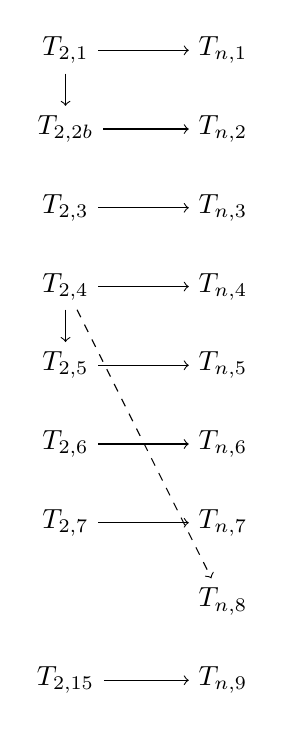
\begin{tikzpicture}
        \node (T2_1) {$T_{2,1}$};
        \node[below of=T2_1] (T2_2) {$T_{2,2b}$};
        \node[below of=T2_2] (T2_3) {$T_{2,3}$};
        \node[below of=T2_3] (T2_4) {$T_{2,4}$};
        \node[below of=T2_4] (T2_5) {$T_{2,5}$};
        \node[below of=T2_5] (T2_6) {$T_{2,6}$};
        \node[below of=T2_6] (T2_7) {$T_{2,7}$};
        % \node[below of=T2_7] (T2_8) {$T_{2,8}$};
        % \node[below of=T2_8] (T2_9) {$T_{2,9}$};
        % \node[below of=T2_9] (T2_10) {$T_{2,10}$};
        % \node[below of=T2_10] (T2_11) {$T_{2,11}$};
        % \node[below of=T2_11] (T2_12) {$T_{2,12}$};
        % \node[below of=T2_12] (T2_13) {$T_{2,13}$};
        % \node[below of=T2_13] (T2_14) {$T_{2,14}$};
        \node[below of=T2_7,yshift=-1cm] (T2_15) {$T_{2,15}$};

        \node[right of=T2_1, xshift=1cm] (Tn_1) {$T_{n,1}$};
        \node[below of=Tn_1] (Tn_2) {$T_{n,2}$};
        \node[below of=Tn_2] (Tn_3) {$T_{n,3}$};
        \node[below of=Tn_3] (Tn_4) {$T_{n,4}$};
        \node[below of=Tn_4] (Tn_5) {$T_{n,5}$};
        \node[below of=Tn_5] (Tn_6) {$T_{n,6}$};
        \node[below of=Tn_6] (Tn_7) {$T_{n,7}$};
        \node[below of=Tn_7] (Tn_8) {$T_{n,8}$};
        \node[below of=Tn_8] (Tn_9) {$T_{n,9}$};

        \draw[->] (T2_1) -- (Tn_1);
        \draw[->] (T2_1) -- (T2_2);
        \draw[->] (T2_2) -- (Tn_2);
        \draw[->] (T2_3) -- (Tn_3);
        \draw[->] (T2_4) -- (Tn_4);
        \draw[->] (T2_4) -- (T2_5);
        \draw[->] (T2_5) -- (Tn_5);
        \draw[->] (T2_6) -- (Tn_6);
        \draw[->] (T2_7) -- (Tn_7);
        \draw[->, dashed] (T2_4) -- (Tn_8);
        \draw[->] (T2_15) -- (Tn_9);
    \end{tikzpicture}
    \caption{Map of standard definitions to their extensions}
    \label{fig:extension-map}
\end{figure}

\subsection{Extension \arabic{extdefctr} of \TotalExtensions\xspace --- Modular Digit Sums}

This definition appears in \cite{Astudillo_2003, Dekking_2023, OEIS-TMS-3-2, Shallit_2022, Shevelev_2017, OEIS-TMS-negabinary, Starosta_2011, Parshina_2017, Robert_2013}.

To extend definition 1 from $2$ to $n$ players, we must first map our concept of parity to base n. We can do this by taking the parity equation defined above and replacing the $2$s with $n$, for $n \in \Integers_{\ge 2}$.

\begin{equation}
    \begin{aligned}
p_n(0) &= 0 \\
p_n(x) &= x + p_n\left(\floor{\dfrac{x}{n}}\right) \pmod{n}
    \end{aligned}
\end{equation}

Under this definition, you can construct the \TMS using the following, starting at 0:

\begin{equation}
    \edef\tempLabel{eq:pn_d\arabic{extdefctr}}
    \label{\tempLabel}
    T_{n,\arabic{extdefctr}}(x, s) = p_s(x)
\end{equation}

Note that this definition is trivially extensible to non-integer bases by redefining $p_n()$, though that is beyond the scope of this paper. This has been done in \cite{OEIS-TMS-3-2, Dekking_2023}. It has also been extended to negative integer bases \cite{OEIS-TMS-negabinary, Shallit_2022, Shevelev_2017}.

Some other works present a more generalized version, where
\begin{equation}
    t_{b,m}(n) = p_b(n) \mod{m}
\end{equation}

This allows for increased flexibility, especially when using fractional bases. In this notation, for negative integer bases, $T_{n,1}(x, s) = p_s(x) \;\; \mod{|s|}$

\subsubsection{Proof of Equivalence with Original Definition \arabic{extdefctr}}

\begin{proof}
It is clear from visual inspection that $p_2$ is identical to our original definition of $p$.

\begin{equation}
    \begin{aligned}
                                                           p_2(x) &= p(x) \\
                         x + p_2\left(\floor{\dfrac{x}{2}}\right) &= x + p\left(\floor{\dfrac{x}{2}}\right) \\
x + \floor{\dfrac{x}{2}} + p_2\left(\floor{\dfrac{x}{2^2}}\right) &= x + \floor{\dfrac{x}{2}} + p\left(\floor{\dfrac{x}{2^2}}\right) \\
       x + \floor{\dfrac{x}{2}} + \floor{\dfrac{x}{2^2}} + \ldots &= x + \floor{\dfrac{x}{2}} + \floor{\dfrac{x}{2^2}} + \ldots
    \end{aligned}
\end{equation}
\end{proof}

This definition is also trivially extended to negative integer bases.

\stepcounter{extdefctr}
\subsection{Extended Definition \arabic{extdefctr} of \TotalExtensions\xspace --- Roots of Unity}

\begin{equation}
    \edef\tempLabel{eq:pn_d\arabic{extdefctr}}
    \label{\tempLabel}
T_{n,\arabic{extdefctr}}(x,s) = \dfrac{\log\left(\omega_s^{p_s(x)}\right)}{\log\left(\omega_s\right)}
\end{equation}

\subsubsection{Proof of Equivalence with Original Definition \arabic{extdefctr}}

\begin{proof}
    Let's start by substituting $s$ for $2$:
    \begin{equation}
    \begin{aligned}
        T_{n,2}(x, 2) &= \dfrac{\log\left(\omega_2^{p_2(x)}\right)}{\log(\omega_2)} \\
                      &= \dfrac{\log\left((-1)^{p_2(x)}\right)}{\log(-1)} \\
                      &= \dfrac{(p_2(x) \mod{2}) \cdot \log(-1)}{\log(-1)} \\
                      &= \dfrac{(p_2(x) \mod{2}) \cdot i\pi}{i\pi} \\
                      &= p_2(x) \mod{2}
    \end{aligned}
    \end{equation}

    This is identical to $T_{2,1}$, which we earlier proved is equivalent to $T_{2,2}$.
\end{proof}

\stepcounter{extdefctr}
\subsection{Extended Definition \arabic{extdefctr} of \TotalExtensions\xspace --- Increment and Extend}

\note{\cite{Cai_2020} gives a good example on how to possibly adapt inversion to incrementing}

In the original version of this definition, we inverted the elements. In base $2$, this is the same thing as adding $1$ (mod $2$). Given that, let $t(x, n)$ be the first $n^x$ elements of the \ETMS, for $n \in \Integers_{\ge 2}$.

\begin{equation}
    \text{inc}(\mathbf{x}, n) = \begin{aligned}[c]
            &x_i + 1 \pmod{n} \\
            &\text{for } \mathbf{x} = (x_0, x_1, \ldots, x_{(|\mathbf{x}|-1)})
    \end{aligned}
\end{equation}

\begin{equation}
    \begin{aligned}
t(0, n) &= \tuple{0} \\
t(1, n) &= \tuple{0, 1, \ldots, n - 1} \\
t(x, n) &= t(x - 1, n) \cdot \text{inc}(t(x - 1, n), n)
    \end{aligned}
\end{equation}

Given the above, we can define a recurrence relation that will give us individual elements. It will be less efficient to compute, but will allow proofs of equivalence to be easier.

\begin{equation}
    \edef\tempLabel{eq:pn_d\arabic{extdefctr}}
    \label{\tempLabel}
    \begin{aligned}
T_{n,\arabic{extdefctr}}(0, s) &= 0 \\
T_{n,\arabic{extdefctr}}(x, s) &= T_{n,\arabic{extdefctr}}\left(x - s^{\floor{\log_s(x)}}, s\right) + 1 \pmod{s}
    \end{aligned}
\end{equation}

\subsubsection{Proof of Equivalence with Original Definition \arabic{extdefctr}} ...

\stepcounter{extdefctr}
\subsection{Extended Definition \arabic{extdefctr} of \TotalExtensions\xspace --- Substitute and Flatten}

This definition appears in \cite{Chen_2019}

\note{There's a bit of a leap here, since we have to explain why the rotation is equivalent to the binary choice presented in the original. There also might be a better syntax to define the rotation, perhaps using the format used in inv and inc.}

\begin{equation}
    \edef\tempLabel{eq:pn_d\arabic{extdefctr}}
    \label{\tempLabel}
    \begin{aligned}
            b(s) &= \tuple{0, 1, \cdots, s - 2, s - 1} \\
r(\mathbf{x}, i) &= \begin{aligned}[c]
                   &\tuple{x_{0 + i \mod{|\mathbf{x}|}}, x_{1 + i \mod{|\mathbf{x}|}}, \ldots} \\
                   &\text{for } \mathbf{x} = \tuple{x_0, x_1, \ldots, x_{(|\mathbf{x}|-1)}}
        \end{aligned} \\
         s(x, s) &= r(b(s), x) \\
            t(0) &= \tuple{0} \\
         t(x, s) &= \bigparallel_{i=0}^{2^{x-1}-1} s(t(x-1)_i, s)  \\
   T_{n,\arabic{extdefctr}}(x, s) &= t(\ceil{\log_s(x + 1)}, s)_x
    \end{aligned}
\end{equation}

% \subsubsection{Musings on Fractional Bases}

% \note{This section is provisional and likely to be cut before publication}

% For the case of base $\tfrac{3}{2}$, I think the way to set it up is to do substitutions as follows:

% \begin{equation}
% \begin{aligned}
%     00 \to 000 \\
%     01 \to 012 \\
%     02 \to 021 \\
%     10 \to 102 \\
%     11 \to 111 \\
%     12 \to 120 \\
%     20 \to 201 \\
%     21 \to 210 \\
%     22 \to 222 \\
% \end{aligned}
% \end{equation}

% So for an example of execution, it would be

% \begin{equation}
%     012 \to 012 \concat 120 = 012120
% \end{equation}

% Of course, I'm not sure that will work since the paper being referenced gives these values as $012201$

% I don't quite know how to generalize this, but it seems to me that all substitutions will follow the following pattern for base $\tfrac{n}{d}$:

% \begin{equation}
% \begin{aligned}
%     w_{0\dots (d-1)} \to w_{0\dots(d-1)} & \concat w_{d\dots (n-1)} \\
%                                          & : p_{\tfrac{n}{d}}\left(w_{0\dots (n-1)}\right) = 0
% \end{aligned}
% \end{equation}

% The difficulty in making this rigorous is going to be deciding how to fill digits $d$ through $n-1$

\subsubsection{Proof of Equivalence with Original Definition \arabic{extdefctr}} ...

\stepcounter{extdefctr}
\subsection{Extended Definition \arabic{extdefctr} of \TotalExtensions\xspace --- Recursive Rotation}

\begin{equation}
    \edef\tempLabel{eq:pn_d\arabic{extdefctr}}
    \label{\tempLabel}
    \begin{aligned}
r(\mathbf{x}, i) &= \begin{aligned}[c]
                   &\tuple{x_{0 + i \mod{|\mathbf{x}|}}, x_{1 + i \mod{|\mathbf{x}|}}, \ldots} \\
                   &\text{for } \mathbf{x} = \tuple{x_0, x_1, \ldots, x_{(|\mathbf{x}|-1)}}
        \end{aligned} \\
         t(0, s) &= \tuple{0} \\
         t(1, s) &= \tuple{0, 1, \ldots, s - 1} \\
         t(x, s) &= \bigparallel_{i=0}^{s-1} r\left(t(x-1, s), i \cdot s^{x-2}\right) \\
   T_{n,\arabic{extdefctr}}(x, s) &= t(\ceil{\log_s(x + 1)}, s)_x
    \end{aligned}
\end{equation}

\subsubsection{Proof of Equivalence with Original Definition \arabic{extdefctr}} ...

\stepcounter{extdefctr}
\subsection{Extended Definition \arabic{extdefctr} of \TotalExtensions\xspace --- Recursion}

\begin{equation}
\begin{aligned}
            T_{n,6}(0, s) &= 0 \\
    T_{n,6}(s \cdot x, s) &= T_{n,6}(x, s) \\
T_{n,6}(s \cdot x + k, s) &= k + T_{n,6}(x, s) \pmod{s}
\end{aligned}
\end{equation}

\subsubsection{Proof of Equivalence with Original Definition \arabic{extdefctr}}

\begin{proof}
    Let's begin by substituting $s$ for $2$:
\begin{equation}
\begin{aligned}
            T_{n,6}(0, 2) &= 0 \\
    T_{n,6}(2 \cdot x, 2) &= T_{n,6}(x, 2) \\
T_{n,6}(2 \cdot x + k, 2) &= k + T_{n,6}(x, 2) \pmod{2}
\end{aligned}
\end{equation}

Note that that only values for $k$ that fit in this definition are $0$ and $1$. This means we can further simplify to:
\begin{equation}
T_{n,6}(2 \cdot x + 1, 2) = 1 + T_{n,6}(x, 2) \pmod{2}
\end{equation}

This is very similar to the definition found in equation \ref{eq:p2_d6}, except that one is adding and the other subtracting. Fortunately, we know that the only values that $T_{2,6}$ will return are $0$ and $1$, which means that these operations will be completely equivalent.

\begin{align*}
1 - 0 \mod{2} &= 1 + 0 \mod{2} \\
1 - 1 \mod{2} &= 1 + 1 \mod{2}
\end{align*}
\end{proof}

\stepcounter{extdefctr}
\subsection{Extended Definition \arabic{extdefctr} of \TotalExtensions\xspace --- Highest Digit Difference}

\begin{equation}
    \edef\tempLabel{eq:pn_d\arabic{extdefctr}}
    \label{\tempLabel}
    \begin{aligned}
\text{XOR}_{n}(a, b) &= \hspace{-13pt} \sum_{i=0}^{\ceil{\log_{n}(\max(a,b) + 1)}} \hspace{-15pt} n^i \left(\floor{\dfrac{a}{n^i}} - \floor{\dfrac{b}{n^i}} \mod{n}\right) \\
       T_{n,\arabic{extdefctr}}(0, s) &= 0 \\
       T_{n,\arabic{extdefctr}}(x, s) &= \begin{aligned}[c]
           &\floor{\log_s(\text{XOR}_{s}(x, x - 1))} \\
           &+ T_{n,\arabic{extdefctr}}(x - 1, s) + 1
       \end{aligned} \pmod{s}
    \end{aligned}
\end{equation}

\note{Substitute n for 2, then simplify, plus a bit}

\subsubsection{Proof of Equivalence with Original Definition \arabic{extdefctr}}

\stepcounter{extdefctr}
\subsection{Extended Definition \arabic{extdefctr} of \TotalExtensions\xspace --- Latin Square Constructions}

This definition appears in \cite{Bolker_2016}\note{, and seemingly only there. It is very clearly equivalent to our Extended Definition 4, but I will need to actually prove that.}

Let $L(n)$ be the reduced-form Latin Square with a first row of $\tuple{0, 1, \dots, n\!-\!1}$, and where each row progresses from one entry to the next as $L(n)_{a,x+1} \equiv L(n)_{a,x} + 1 \pmod{n}$. For each iteration $t_n$, substitute each entry $x$ for the string $L(n)_{x,*}$.

\note{Needs more explanation, largely copying from std def 3}

\begin{equation}
L(N) = \begin{pmatrix}
0 & 1 & 2 & \dots & N\!\!-\!\!1 \\
1 & 2 & \ddots & N\!\!-\!\!1 & 0 \\
2 & \ddots & N\!\!-\!\!1 & 0 & 1 \\
\vdots & N\!\!-\!\!1 & 0 & 1 & \ddots \\
N\!\!-\!\!1& 0 & 1 & \ddots & \ddots
\end{pmatrix}
\end{equation}

\subsubsection{Proof of Equivalence with Original Definition 4}

\stepcounter{extdefctr}
\subsection{Extended Definition \arabic{extdefctr} of \TotalExtensions\xspace --- Generating Functions}

\begin{equation}
\begin{aligned}
    G_s(x) &= \mathcal{G.F.} \;\; \begin{aligned}    
    \prod_{k\ge0}^\infty \sum_{i=0}^{s-1} \omega_s^i \cdot x^{i \cdot s^k}
    \end{aligned} \\
    \omega_s ^{T_{n,\arabic{extdefctr}}(j, s)} &= [x^j]G_s(x) \\
    T_{n,\arabic{extdefctr}}(j, s) &= \dfrac{\log\left([x^j]G_s(x)\right)}{\log(\omega_s)} \\
              &= \dfrac{\log\left([x^j]G_x(x)\right) \cdot s}{2i\pi} \\
\end{aligned}
\end{equation}

\subsubsection{Proof of Equivalence with Original Definition 15}

\begin{proof}
\textbf{Observation 1}: to start, let us rephrase definition 15 slightly

\begin{equation}
\begin{aligned}
T_{2,15}(n) &= [x^n]G(x) \\
    &= [x^n] \left(\begin{aligned}[c]
    \dfrac{\displaystyle\sum_{k\ge0}^\infty x^k - \prod_{k \ge 0}^\infty (1 - x^{2^k})}{2}
    \end{aligned}\right) \\
    &= \dfrac{[x^n] \left(\begin{aligned}[c]
    \displaystyle\sum_{k\ge0}^\infty x^k - \prod_{k \ge 0}^\infty (1 - x^{2^k})\end{aligned}\right)}{2}
     \\
    &= \dfrac{1 - [x^n]\begin{aligned}[c]
    \displaystyle\prod_{k \ge 0}^\infty (1 - x^{2^k})
    \end{aligned}
    }{2}
\end{aligned}
\end{equation}

\textbf{Observation 2}: the aparatus around the infinite product exists entirely to translate $\{1, -1\} \to \{0, 1\}$. Another way to do that is to take the complex log of this output: for $x = \{1, -1\}: \tfrac{\log(x)}{\log(-1)} = \{0, 1\}$

\textbf{Inference 1}: \begin{equation}
    \dfrac{1 - [x^n]\begin{aligned}
    \displaystyle\prod_{k \ge 0}^\infty (1 - x^{2^k})
    \end{aligned}
    }{2} = \dfrac{\log\left([x^n]\begin{aligned}
    \displaystyle\prod_{k \ge 0}^\infty (1 - x^{2^k})
    \end{aligned}\right)}{\log(-1)}
\end{equation}

\textbf{Observation 3}: $\omega_2 = -1$

\textbf{Observation 4}: If we take $T_{n,\arabic{extdefctr}}(x, s)$ for $s=2$, we get \begin{equation}
\begin{aligned}
    G_2(x) &= \mathcal{G.F.} \;\; \begin{aligned}    
    \prod_{k\ge0}^\infty \sum_{i=0}^{2-1} \omega_2^i \cdot x^{i \cdot 2^k}
    \end{aligned} \\
           &= \mathcal{G.F.} \;\; \begin{aligned}    
    \prod_{k\ge0}^\infty \omega_2^0 \cdot x^{0 \cdot 2^k} + \omega_2^i \cdot x^{i \cdot 2^k}
    \end{aligned} \\
           &= \mathcal{G.F.} \;\; \begin{aligned}    
    \prod_{k\ge0}^\infty 1 + (-1) \cdot x^{2^k}
    \end{aligned} \\
           &= \mathcal{G.F.} \;\; \begin{aligned}    
    \prod_{k\ge0}^\infty 1 - x^{2^k}
    \end{aligned}
\end{aligned}
\end{equation}
This is identical to the product found in $T_{2,15}$.

\textbf{Conclusion}: $T_{n,\arabic{extdefctr}}(x, s) = T_{2,15}(x)$
\end{proof}

\subsection{Summary}

Of the \TotalExtensions we discussed above:
\begin{itemize}
    % discovery source
    \item 1 was found on the OEIS ($T_{n,1}$)
    \item 2 were found in another paper ($T_{n,4}, T_{n,8}$)
    \item 6 are original to this paper ($T_{n,2\dots3}, T_{n,5\dots7}, T_{n,9}$)
    \\% generating method
    \item 7 utilize recursion ($T_{n,1\dots7}$)
    \item 4 utilize floor-division ($T_{n,1\dots2}, T_{n,6\dots7}$)
    \item 4 use operations on strings, not integers ($T_{2,3\dots5}, T_{n,8}$)
    \item 0 have closed form solutions
\end{itemize}

\section{Proving Equivalence Between Extended Definitions}

All definitions are tested computationally, though due to resource limitations, to different extents.

\renewcommand{\arraystretch}{1.25}
\begin{table}[H]
\label{tab:testing_bn}
\caption{Extent of Testing in Integer Bases $> 2$}
\centering
\begin{tabular}{|l|c|r|}
\hline
\textbf{Definition}       & \textbf{Bases}         & \textbf{Entries Tested}            \\\hline
$T_{n,1}$                 & 3 - 256                & $2^{30} = 1,073,741,824$           \\\hline
\multirow{2}{*}{$T_{n,2}$}& 3 - 16                 & $2^{29} = 536,870,912$             \\\cline{2-3}
                          & 17 - 256               &\multirow{4}{*}{$2^{30}=1,073,741,824$}\\\cline{1-2}
\multirow{6}{*}{$T_{n,3}$}& 3 - 16                 &                                    \\\cline{2-2} 
                          & 33 - 48                &                                    \\\cline{2-2} 
                          & 65 - 208               &                                    \\\cline{2-3} 
                          & 17 - 32                &\multirow{3}{*}{$2^{29}=536,870,912$}\\\cline{2-2}
                          & 49 - 64                &                                    \\\cline{2-2}
                          & 209 - 256              &                                    \\\hline
\multirow{5}{*}{$T_{n,4}$}& 3 - 16                 &\multirow{3}{*}{$2^{30}=1,073,741,824$}\\\cline{2-2}
                          & 33 - 48                &                                    \\\cline{2-2}
                          & 65 - 256               &                                    \\\cline{2-3}
                          & 17 - 32                &\multirow{4}{*}{$2^{29}=536,870,912$}\\\cline{2-2} 
                          & 49 - 64                &                                    \\\cline{1-2}
\multirow{4}{*}{$T_{n,5}$}& 3 - 48                 &                                    \\\cline{2-2}
                          & 65 - 192               &                                    \\\cline{2-3}
                          & 49 - 64                &\multirow{2}{*}{$2^{28}=268,435,456$}\\\cline{2-2}
                          & 193 - 256              &                                    \\\hline
$T_{n,6}$                 &\multirow{2}{*}{3 - 256}&\multirow{4}{*}{$2^{30}=1,073,741,824$}\\\cline{1-1}
$T_{n,7}$                 &                        &                                    \\\cline{1-2}
\multirow{3}{*}{$T_{n,8}$}& 3 - 32                 &                                    \\\cline{2-2}
                          & 49 - 256               &                                    \\\cline{2-3}
                          & 33 - 48                & $2^{29} = 536,870,912$             \\\hline
\multirow{2}{*}{$T_{n,9}$}& 3 - 80                 & $2^{10} = 1,024$                   \\\cline{2-3}
                          & 81 - 256               & $2^{11} = 2,048$                   \\\hline
\end{tabular}
\end{table}

\begin{table}[H]
\label{tab:comparison-bn}
\centering
\caption{Comparison Matrix of the Extended Definitions}
\note{X = done, O = target} \\
\begin{tabular}{|c|c|c|c|c|c|c|c|c|}
\cline{1-1}
\!1\!\\ \cline{1-2}
\!X\!&\!2\!\\ \cline{1-3}
\!O\!&     &\!3\!\\ \cline{1-4}
     &     &\!O\!&\!4\!\\ \cline{1-5}
     &     &     &\!O\!&\!5\!\\ \cline{1-6}
\!O\!&     &     &     &     &\!6\!\\ \cline{1-7}
\!O\!&     &     &     &     &     &\!7\!\\ \cline{1-8}
     &     &\!X\!&     &     &     &     &\!8\!\\ \cline{1-9}
\!O\!&     &     &     &     &     &     &     &\!9\!\\ \hline
\end{tabular}
\end{table}
\renewcommand{\arraystretch}{1}

\subsection{Correlating Definition 1 and Definition 2}

\begin{proof}
\par\noindent\par
    \textbf{Observation 1}: For all integers $n$, $\omega_s^n = \omega_s^{n \; \mod{s}}$

    \textbf{Inference 1}: $\dfrac{\log(\omega_s^n)}{\log(\omega_s)} = n \; \mod{s}$

    \textbf{Conclusion}: \begin{equation}
        \begin{aligned}
            T_{n,2}(x, s) &= \dfrac{\log(\omega_s^{p_s(x)})}{\log(\omega_s)} \\
                          &= \dfrac{(p_s(x) \; \mod{s}) \cdot \log(\omega_s)}{\log(\omega_s)} \\
                          &= \dfrac{(p_s(x) \; \mod{s}) \cdot 2i\pi s^{-1}}{2i\pi s^{-1}} \\
                          &= p_s(x) \; \mod{s} \\
                          &= T_{n,1}(x, s)
        \end{aligned}
    \end{equation}
\end{proof}

\subsection{Correlating Definition 4 and Definition 8}

\begin{proof}
\par\noindent\par
    \textbf{Observation 1}: For any given row of $L(N)$, it will start with the index of the row

    \textbf{Observation 2}: For any given row of $L(N)$, it will end with 1 less than the index of the row $\pmod{N}$

    \textbf{Inference 1}: $L(N)_{x,*} = r(b(N), x)$

    \textbf{Observation 3}: $T_{n,4}$ is defined as substituting $r(b(N),x)$ for each element $x$ in the previous iteration

    \textbf{Conclusion}: $T_{n,4} = T_{n,8}$
\end{proof}

\subsection{Summary}

\section{Proving Persistence (Or Lack Thereof) of Original Properties}

\subsection{Use as a Fair-Share Sequence}

\note{Goal: show that for a variety of value functions, greedy algorithms given this turn order will always minimize inequality. They should at least do so more than the standard turn order. This is going to look like setting up an equation to show}

\begin{equation}
\begin{aligned}
             eq(x, y) &= \begin{cases}
                     1& \text{if } x = y \\
                     0& \text{if } x \ne y
              \end{cases} \\
           f(v, p, s) &= \lim_{n \to \infty} \sum_{i=0}^n v(i) \cdot eq(T_n(i, s), p) \\
        \forall p : p &\in \{1, \dots, s-1\}\\
f(v, 0, s) + \epsilon &< f(v, p, s) < f(v, 0, s) - \epsilon
\end{aligned}
\end{equation}

\note{This is for $v(i)$ being a value function and $\epsilon$ being an arbitrarily small number. $f()$ is therefore the sum of total value that they will be receiving. For example, one could model a board game as $v(i) = \tfrac{1}{2^i}$, where $v()$ models the amount each turn contributes to your probability of victory. Note that this may be very hard to show for versions of $v()$ which shrink too quickly, such as $v(i) = \tfrac{1}{i!}$, so for those cases we must show that it's better than the standard turn order}

\subsubsection{On the value function of 1}

It is well known \cite{Cai_2020} for the Standard \TMS that
\begin{equation}
    \lim_{n\to\infty} \sum_{i=0}^n \dfrac{T_{2}(i)}{n+1} = \dfrac{1}{2}
\end{equation}

\note{Does this generalize to: ?}

\begin{equation}
    \lim_{n\to\infty} \sum_{i=0}^n\dfrac{T_{n}(i, s)}{n+1} = \sum_{i=0}^{s-1}\dfrac{i}{s} = \dfrac{n-1}{2}
\end{equation}

\note{and}

\begin{equation}
\begin{aligned}
    &\forall{x} \;|\; 0 \le x < s \text{ and } x \in \mathbf{Z} \\
    &\lim_{n\to\infty} \sum_{i=0}^n\dfrac{eq\left(T_{n}(i, s), x\right)}{n+1} = \dfrac{1}{s}
\end{aligned}
\end{equation}

\subsubsection{On more general value functions}

\subsection{Aperiodicity}

\note{Not totally sure how this should go, but I think a good approximation would be to show that the distance between the nearest two appearances of a substring grows to infinity much faster than the length of those substrings grows}

\subsection{Palindrome}

This seems trivially violated for $n > 2$. Example: $t_3(2) = \tuple{0, 1, 2, 1, 2, 0, 2, 0, 1}$

This doesn't even work for power-of-2 bases, like $t_4(2) = \tuple{0, 1, 2, 3, 1, 2, 3, 0, 2, 3, 0, 1, 3, 0, 1, 2}$

\note{I am unable to think of any base other than 2 where this property could even conceivably hold true. Probably need to do a proof by contradiction, assuming base $\ge3$}

\subsection{Uniform Recurrence}

\note{The \TMS is a uniformly recurrent word: given any finite string X in the sequence, there is some length nX (often much longer than the length of X) such that X appears in every block of length nX}

\section{Acknowledgment}

We thank Dan Rowe for helping with the initial work on this paper, as well as Randy Appleton and Lydia Crocker who helped greatly with proofreading and editing.

\section{Appendix}

\subsection{General Performance Results}

\begin{figure}[H]
    \centering
    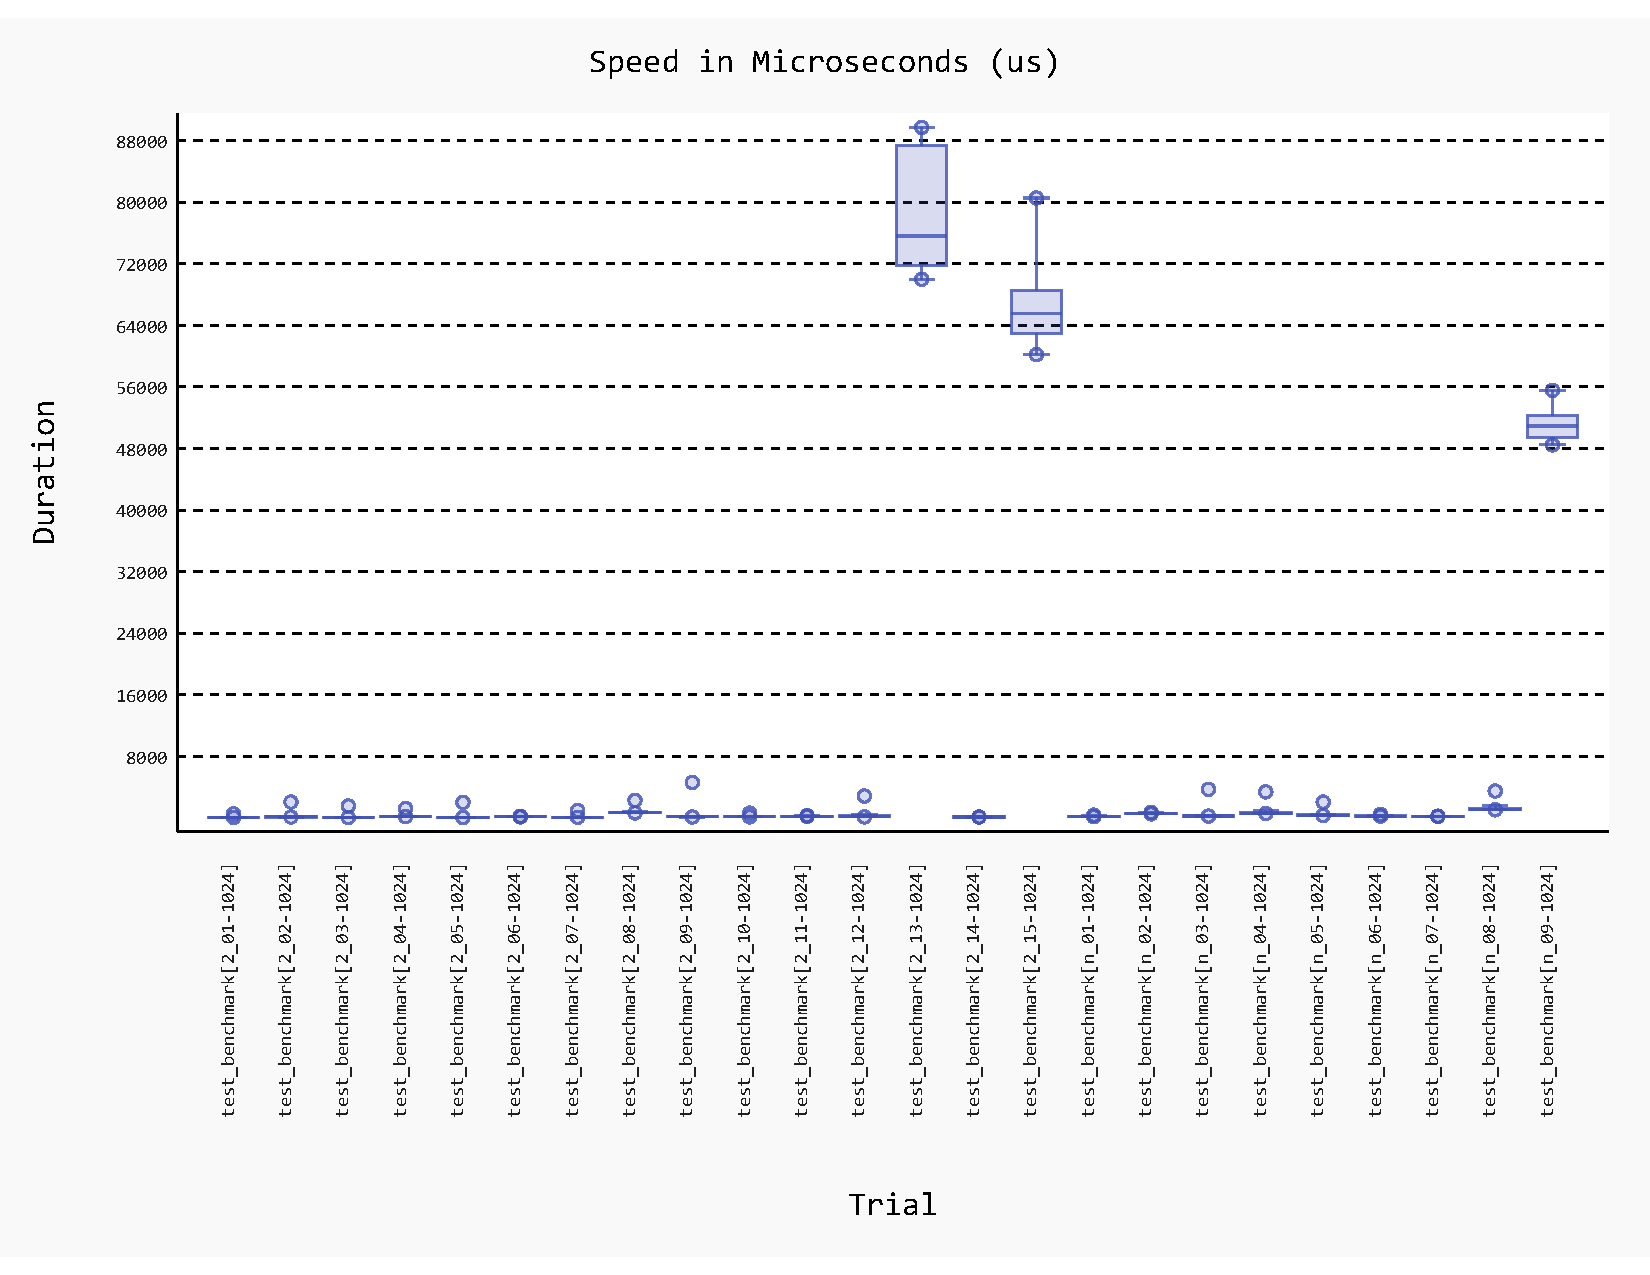
\includegraphics[width=\linewidth]{figures/benchmark/20241122_154339.pdf}
    \caption{Benchmark results up to seconds.}
    \label{fig:benchmark_in_s}
\end{figure}

\begin{figure}[H]
    \centering
    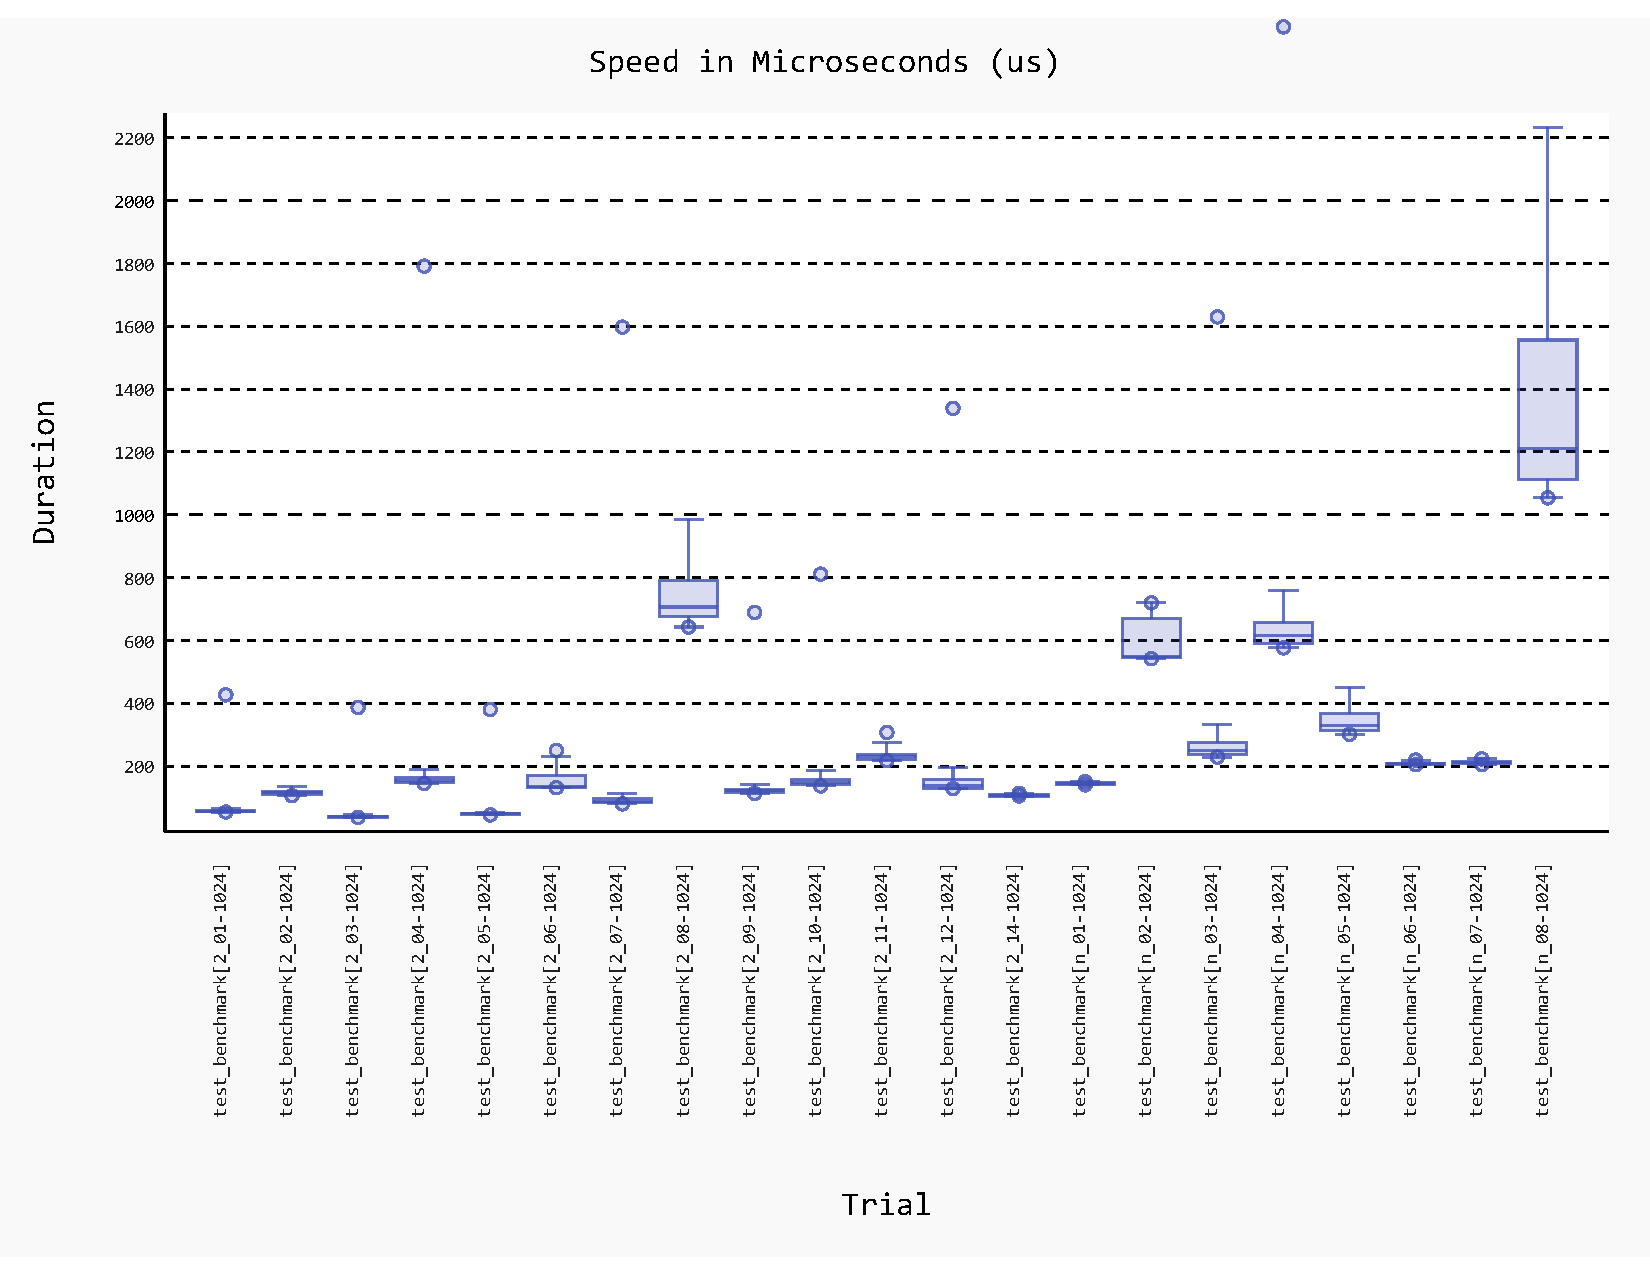
\includegraphics[width=\linewidth]{figures/benchmark/20241122_163356.pdf}
    \caption{Benchmark results up to milliseconds.}
    \label{fig:benchmark_in_ms}
\end{figure}

\note{These figures are temporary and will be replaced with something prettier when things are finalized}

\setcounter{stddefctr}{1}
\setcounter{extdefctr}{1}

\subsection{Complexity of Original Definition \arabic{stddefctr}}
\edef\tempLabel{ca:p2_d\arabic{stddefctr}}
\expandafter\label\expandafter\tempLabel

\subsubsection{Time Complexity}

In an idealized case, this definition will simplify to:

\begin{equation}
T_{2,\arabic{stddefctr}}(n) = \left(\sum_{i=0}^{\ceil{\log_2(n + 1)}} \hspace{-8pt} \floor{\dfrac{n}{2^i} \mod{2}} \right) \mod{2}
\end{equation}

This is pretty explicitly $O(\log(n))$ operations. This means that generating the first $n$ entries will take $O(n\log(n))$ operations.

In languages with dynamically sized integers, this can be slightly more complicated. In the above, we perform $\log(n)$ bit shifts, multiplications, moduli, and additions. Since a bit shift is constant time, calculation will be dominated by multiplication, division, and moduli. Each of these take $O(\log(n) \cdot \log(\log(n)))$, where $n$ is the largest number involved. This means that in such languages, we can expect it to take $O(\log(n)^2 \cdot \log(\log(n)))$ operations per element, for $O(n \cdot \log(n)^2 \cdot \log(\log(n)))$ in total.

\renewcommand{\arraystretch}{1.25}
\begin{table}[H]
    \centering
    \caption{Time Complexity Summary of Standard Definition \arabic{stddefctr}}
    \begin{tabular}{|c|c|c|}
        \hline
        & \textbf{Fixed Size} & \textbf{Arbitrary Size} \\
        \hline
        \textbf{Per Element} & $O(\log(n))$ & $O(\log(n)^2 \cdot \log(\log(n)))$ \\
        \hline
        \textbf{In Total} & $O(n \cdot \log(n))$ & $O(n \cdot \log(n)^2 \cdot \log(\log(n)))$ \\
        \hline
    \end{tabular}
    \edef\tempLabel{tab:time_p2_d\arabic{stddefctr}}
     \expandafter\label\expandafter\tempLabel
\end{table}
\renewcommand{\arraystretch}{1}

\subsubsection{Space Complexity}

This is one of the more space-efficient implementations. Each element takes at most the same size as the passed integer. In languages that use Fixed Size integers, that means it will take $O(1)$ space. In languages like Python that use Arbitrary Size integers, it would take $O(\log(n))$ space, where $n$ is the largest element you intend to calculate. If you intend to store all $n$ elements, it will therefore take $O(n)$ or $O(n \cdot \log(n))$ space.

\begin{table}[H]
    \centering
    \caption{Space Complexity Summary of Standard Definition \arabic{stddefctr}}
    \begin{tabular}{|c|c|c|}
        \hline
        & \textbf{Fixed Size} & \textbf{Arbitrary Size} \\
        \hline
        \textbf{Per Element} & $O(1)$ & $O(\log(n))$ \\
        \hline
        \textbf{In Total} & $O(n)$ & $O(n \cdot \log(n))$ \\
        \hline
    \end{tabular}
    \edef\tempLabel{tab:space_p2_d\arabic{stddefctr}}
     \expandafter\label\expandafter\tempLabel
\end{table}

\stepcounter{stddefctr}
\subsection{Complexity of Original Definition \arabic{stddefctr}}
\edef\tempLabel{ca:p2_d\arabic{stddefctr}}
 \expandafter\label\expandafter\tempLabel

\subsubsection{Time Complexity} ...

\begin{table}[H]
    \centering
    \caption{Time Complexity Summary of Standard Definition \arabic{stddefctr}}
    \begin{tabular}{|c|c|c|}
        \hline
        & \textbf{Fixed Size} & \textbf{Arbitrary Size} \\
        \hline
        \textbf{Per Element} &  &  \\
        \hline
        \textbf{In Total} &  &  \\
        \hline
    \end{tabular}
    \edef\tempLabel{tab:time_p2_d\arabic{stddefctr}}
     \expandafter\label\expandafter\tempLabel
\end{table}

\subsubsection{Space Complexity} ...

\begin{table}[H]
    \centering
    \caption{Space Complexity Summary of Standard Definition \arabic{stddefctr}}
    \begin{tabular}{|c|c|c|}
        \hline
        & \textbf{Fixed Size} & \textbf{Arbitrary Size} \\
        \hline
        \textbf{Per Element} &  &  \\
        \hline
        \textbf{In Total} &  &  \\
        \hline
    \end{tabular}
    \edef\tempLabel{tab:space_p2_d\arabic{stddefctr}}
     \expandafter\label\expandafter\tempLabel
\end{table}

\stepcounter{stddefctr}
\subsection{Complexity of Original Definition \arabic{stddefctr}}
\edef\tempLabel{ca:p2_d\arabic{stddefctr}}
 \expandafter\label\expandafter\tempLabel

\subsubsection{Time Complexity} ...

\begin{table}[H]
    \centering
    \caption{Time Complexity Summary of Standard Definition \arabic{stddefctr}}
    \begin{tabular}{|c|c|c|}
        \hline
        & \textbf{Fixed Size} & \textbf{Arbitrary Size} \\
        \hline
        \textbf{Per Element} &  &  \\
        \hline
        \textbf{In Total} &  &  \\
        \hline
    \end{tabular}
    \edef\tempLabel{tab:time_p2_d\arabic{stddefctr}}
     \expandafter\label\expandafter\tempLabel
\end{table}

\subsubsection{Space Complexity} ...

\begin{table}[H]
    \centering
    \caption{Space Complexity Summary of Standard Definition \arabic{stddefctr}}
    \begin{tabular}{|c|c|c|}
        \hline
        & \textbf{Fixed Size} & \textbf{Arbitrary Size} \\
        \hline
        \textbf{Per Element} &  &  \\
        \hline
        \textbf{In Total} &  &  \\
        \hline
    \end{tabular}
    \edef\tempLabel{tab:space_p2_d\arabic{stddefctr}}
     \expandafter\label\expandafter\tempLabel
\end{table}

\stepcounter{stddefctr}
\subsection{Complexity of Original Definition \arabic{stddefctr}}
\edef\tempLabel{ca:p2_d\arabic{stddefctr}}
 \expandafter\label\expandafter\tempLabel

\subsubsection{Time Complexity} ...

\begin{table}[H]
    \centering
    \caption{Time Complexity Summary of Standard Definition \arabic{stddefctr}}
    \begin{tabular}{|c|c|c|}
        \hline
        & \textbf{Fixed Size} & \textbf{Arbitrary Size} \\
        \hline
        \textbf{Per Element} &  &  \\
        \hline
        \textbf{In Total} &  &  \\
        \hline
    \end{tabular}
    \edef\tempLabel{tab:time_p2_d\arabic{stddefctr}}
     \expandafter\label\expandafter\tempLabel
\end{table}

\subsubsection{Space Complexity} ...

\begin{table}[H]
    \centering
    \caption{Space Complexity Summary of Standard Definition \arabic{stddefctr}}
    \begin{tabular}{|c|c|c|}
        \hline
        & \textbf{Fixed Size} & \textbf{Arbitrary Size} \\
        \hline
        \textbf{Per Element} &  &  \\
        \hline
        \textbf{In Total} &  &  \\
        \hline
    \end{tabular}
    \edef\tempLabel{tab:space_p2_d\arabic{stddefctr}}
     \expandafter\label\expandafter\tempLabel
\end{table}

\stepcounter{stddefctr}
\subsection{Complexity of Original Definition \arabic{stddefctr}}
\edef\tempLabel{ca:p2_d\arabic{stddefctr}}
 \expandafter\label\expandafter\tempLabel

\subsubsection{Time Complexity} ...

\begin{table}[H]
    \centering
    \caption{Time Complexity Summary of Standard Definition \arabic{stddefctr}}
    \begin{tabular}{|c|c|c|}
        \hline
        & \textbf{Fixed Size} & \textbf{Arbitrary Size} \\
        \hline
        \textbf{Per Element} &  &  \\
        \hline
        \textbf{In Total} &  &  \\
        \hline
    \end{tabular}
    \edef\tempLabel{tab:time_p2_d\arabic{stddefctr}}
     \expandafter\label\expandafter\tempLabel
\end{table}

\subsubsection{Space Complexity} ...

\begin{table}[H]
    \centering
    \caption{Space Complexity Summary of Standard Definition \arabic{stddefctr}}
    \begin{tabular}{|c|c|c|}
        \hline
        & \textbf{Fixed Size} & \textbf{Arbitrary Size} \\
        \hline
        \textbf{Per Element} &  &  \\
        \hline
        \textbf{In Total} &  &  \\
        \hline
    \end{tabular}
    \edef\tempLabel{tab:space_p2_d\arabic{stddefctr}}
     \expandafter\label\expandafter\tempLabel
\end{table}

\stepcounter{stddefctr}
\subsection{Complexity of Original Definition \arabic{stddefctr}}
\edef\tempLabel{ca:p2_d\arabic{stddefctr}}
 \expandafter\label\expandafter\tempLabel

\subsubsection{Time Complexity}

At each step in calculation, the value of $n$ passed to the next recursion is halved. This means that it will take $O(\log_2(n))$ recursive steps. Each recursion involves at maximum 2 subtractions and a bit shift. In most languages with Fixed Size integers, this will take constant time. However, in languages with Arbitrary Size integers these subtractions will typically take $O(\log(n))$, where $n$ is the largest integer in the operation. This means we can expect it to take $O(\log(n)^2$ operations.

\renewcommand{\arraystretch}{1.25}
\begin{table}[H]
    \centering
    \caption{Time Complexity Summary of Standard Definition \arabic{stddefctr}}
    \begin{tabular}{|c|c|c|}
        \hline
        & \textbf{Fixed Size} & \textbf{Arbitrary Size} \\
        \hline
        \textbf{Per Element} & $O(\log(n))$ & $O(\log(n)^2)$ \\
        \hline
        \textbf{In Total} & $O(n \cdot \log(n))$ & $O(n \cdot \log(n)^2)$ \\
        \hline
    \end{tabular}
    \edef\tempLabel{tab:time_p2_d\arabic{stddefctr}}
     \expandafter\label\expandafter\tempLabel
\end{table}
\renewcommand{\arraystretch}{1}

\subsubsection{Space Complexity}

This is one of the more space-efficient implementations. Each element takes at most the same size as the passed integer. In languages that use Fixed Size integers, that means it will take $O(1)$ space. In languages like Python that use Arbitrary Size integers, it would take $O(\log(n))$ space, where $n$ is the largest element you intend to calculate. If you intend to store all $n$ elements, it will therefore take $O(n)$ or $O(n \cdot \log(n))$ space.

\begin{table}[H]
    \centering
    \caption{Space Complexity Summary of Standard Definition \arabic{stddefctr}}
    \begin{tabular}{|c|c|c|}
        \hline
        & \textbf{Fixed Size} & \textbf{Arbitrary Size} \\
        \hline
        \textbf{Per Element} & $O(1)$ & $O(\log(n))$ \\
        \hline
        \textbf{In Total} & $O(n)$ & $O(n \cdot \log(n))$ \\
        \hline
    \end{tabular}
    \edef\tempLabel{tab:space_p2_d\arabic{stddefctr}}
     \expandafter\label\expandafter\tempLabel
\end{table}

\stepcounter{stddefctr}
\subsection{Complexity of Original Definition \arabic{stddefctr}}
\edef\tempLabel{ca:p2_d\arabic{stddefctr}}
 \expandafter\label\expandafter\tempLabel

\subsubsection{Time Complexity}

\note{Since this algorithm works sequentially, and cannot perform computation of an arbitrary element without recursing to the base case, the time is equal on a per-element and in-total basis}

\renewcommand{\arraystretch}{1.25}
\begin{table}[H]
    \centering
    \caption{Time Complexity Summary of Standard Definition \arabic{stddefctr}}
    \begin{tabular}{|c|c|c|}
        \hline
        & \textbf{Fixed Size} & \textbf{Arbitrary Size} \\
        \hline
        \textbf{Per Element} & $O(n \cdot \log(n))$ & $O\left(n \cdot \log(n)^2\right)$ \\
        \hline
        \textbf{In Total} & $O(n \cdot \log(n))$ & $O\left(n \cdot \log(n)^2\right)$ \\
        \hline
    \end{tabular}
    \edef\tempLabel{tab:time_p2_d\arabic{stddefctr}}
     \expandafter\label\expandafter\tempLabel
\end{table}
\renewcommand{\arraystretch}{1}

\subsubsection{Space Complexity} ...

\begin{table}[H]
    \centering
    \caption{Space Complexity Summary of Standard Definition \arabic{stddefctr}}
    \begin{tabular}{|c|c|c|}
        \hline
        & \textbf{Fixed Size} & \textbf{Arbitrary Size} \\
        \hline
        \textbf{Per Element} & $O(1)$ & $O(\log(n))$ \\
        \hline
        \textbf{In Total} & $O(n)$ & $O(n \cdot \log(n))$ \\
        \hline
    \end{tabular}
    \edef\tempLabel{tab:space_p2_d\arabic{stddefctr}}
     \expandafter\label\expandafter\tempLabel
\end{table}

\stepcounter{stddefctr}
\subsection{Complexity of Original Definition \arabic{stddefctr}}
\edef\tempLabel{ca:p2_d\arabic{stddefctr}}
 \expandafter\label\expandafter\tempLabel

\subsubsection{Time Complexity}

\note{memoization doesn't seem to help in the worst case of $1\ldots1_2$, so you should still end up calculating the value of $b()$ for every positive number less than $n$}

\renewcommand{\arraystretch}{1.25}
\begin{table}[H]
    \centering
    \caption{Time Complexity Summary of Standard Definition \arabic{stddefctr}}
    \begin{tabular}{|c|c|c|}
        \hline
        & \textbf{Fixed Size} & \textbf{Arbitrary Size} \\
        \hline
        \textbf{Per Element} & $O(n)$ & $O(n \cdot \log(n) \cdot \log(\log(n)))$ \\
        \hline
        \textbf{In Total} & $O\left(n^2\right)$ & $O\left(n^2 \cdot \log(n) \cdot \log(\log(n))\right)$ \\
        \hline
    \end{tabular}
    \edef\tempLabel{tab:time_p2_d\arabic{stddefctr}}
     \expandafter\label\expandafter\tempLabel
\end{table}

\subsubsection{Space Complexity}

There are two ways to implement this algorithm in terms of space complexity. They both have equal worst-case time complexity. The first is to take the recursive approach, and the second is to use dynamic programming.

In a recursive approach, you will end up descending $O(\log(n))$ stack frames, each of which will contain at minimum 1 integer. In the dynamic approach, you will keep a table of all the values of $b()$ from $0$ through $n$. The biggest difference between these approaches is that in the recursive approach you may need to repeat calculations.

\begin{table}[H]
    \centering
    \caption{Space Complexity Summary of Standard Definition \arabic{stddefctr}}
    \begin{tabular}{|cc|c|c|}
        \hline
        & & \textbf{Fixed Size} & \textbf{Arbitrary Size} \\
        \hline
        \multirow{2}{*}{\textbf{Recursive}} \hspace{-5pt} & \textbf{Per Element} & $O(\log(n))$ & $O(n \cdot \log(n))$ \\
        \cline{2-4}
        & \textbf{In Total} & $O(n \cdot \log(n))$ & $O\left(n^2 \cdot \log(n)\right)$ \\
        \hline
        \multirow{2}{*}{\textbf{Dynamic}} \hspace{-5pt} & \textbf{Per Element} & $O(n)$ & $O(n \cdot \log(n))$ \\
        \cline{2-4}
        & \textbf{In Total} & $O\left(n^2\right)$ & $O\left(n^2 \cdot \log(n)\right)$ \\
        \hline
    \end{tabular}
    \edef\tempLabel{tab:space_p2_d\arabic{stddefctr}}
     \expandafter\label\expandafter\tempLabel
\end{table}
\renewcommand{\arraystretch}{1}

\stepcounter{stddefctr}
\subsection{Complexity of Original Definition \arabic{stddefctr}}
\edef\tempLabel{ca:p2_d\arabic{stddefctr}}
 \expandafter\label\expandafter\tempLabel

\subsubsection{Time Complexity} ...

\begin{table}[H]
    \centering
    \caption{Time Complexity Summary of Standard Definition \arabic{stddefctr}}
    \begin{tabular}{|c|c|c|}
        \hline
        & \textbf{Fixed Size} & \textbf{Arbitrary Size} \\
        \hline
        \textbf{Per Element} &  &  \\
        \hline
        \textbf{In Total} &  &  \\
        \hline
    \end{tabular}
    \edef\tempLabel{tab:time_p2_d\arabic{stddefctr}}
     \expandafter\label\expandafter\tempLabel
\end{table}

\subsubsection{Space Complexity} ...

\begin{table}[H]
    \centering
    \caption{Space Complexity Summary of Standard Definition \arabic{stddefctr}}
    \begin{tabular}{|c|c|c|}
        \hline
        & \textbf{Fixed Size} & \textbf{Arbitrary Size} \\
        \hline
        \textbf{Per Element} &  &  \\
        \hline
        \textbf{In Total} &  &  \\
        \hline
    \end{tabular}
    \edef\tempLabel{tab:space_p2_d\arabic{stddefctr}}
     \expandafter\label\expandafter\tempLabel
\end{table}

\stepcounter{stddefctr}
\subsection{Complexity of Original Definition \arabic{stddefctr}}
\edef\tempLabel{ca:p2_d\arabic{stddefctr}}
 \expandafter\label\expandafter\tempLabel

\subsubsection{Time Complexity} ...

\begin{table}[H]
    \centering
    \caption{Time Complexity Summary of Standard Definition \arabic{stddefctr}}
    \begin{tabular}{|c|c|c|}
        \hline
        & \textbf{Fixed Size} & \textbf{Arbitrary Size} \\
        \hline
        \textbf{Per Element} &  &  \\
        \hline
        \textbf{In Total} &  &  \\
        \hline
    \end{tabular}
    \edef\tempLabel{tab:time_p2_d\arabic{stddefctr}}
     \expandafter\label\expandafter\tempLabel
\end{table}

\subsubsection{Space Complexity} ...

\begin{table}[H]
    \centering
    \caption{Space Complexity Summary of Standard Definition \arabic{stddefctr}}
    \begin{tabular}{|c|c|c|}
        \hline
        & \textbf{Fixed Size} & \textbf{Arbitrary Size} \\
        \hline
        \textbf{Per Element} &  &  \\
        \hline
        \textbf{In Total} &  &  \\
        \hline
    \end{tabular}
    \edef\tempLabel{tab:space_p2_d\arabic{stddefctr}}
     \expandafter\label\expandafter\tempLabel
\end{table}

\stepcounter{stddefctr}
\subsection{Complexity of Original Definition \arabic{stddefctr}}
\edef\tempLabel{ca:p2_d\arabic{stddefctr}}
 \expandafter\label\expandafter\tempLabel

\subsubsection{Time Complexity} ...

\begin{table}[H]
    \centering
    \caption{Time Complexity Summary of Standard Definition \arabic{stddefctr}}
    \begin{tabular}{|c|c|c|}
        \hline
        & \textbf{Fixed Size} & \textbf{Arbitrary Size} \\
        \hline
        \textbf{Per Element} &  &  \\
        \hline
        \textbf{In Total} &  &  \\
        \hline
    \end{tabular}
    \edef\tempLabel{tab:time_p2_d\arabic{stddefctr}}
     \expandafter\label\expandafter\tempLabel
\end{table}

\subsubsection{Space Complexity} ...

\begin{table}[H]
    \centering
    \caption{Space Complexity Summary of Standard Definition \arabic{stddefctr}}
    \begin{tabular}{|c|c|c|}
        \hline
        & \textbf{Fixed Size} & \textbf{Arbitrary Size} \\
        \hline
        \textbf{Per Element} &  &  \\
        \hline
        \textbf{In Total} &  &  \\
        \hline
    \end{tabular}
    \edef\tempLabel{tab:space_p2_d\arabic{stddefctr}}
     \expandafter\label\expandafter\tempLabel
\end{table}

\stepcounter{stddefctr}
\subsection{Complexity of Original Definition \arabic{stddefctr}}
\edef\tempLabel{ca:p2_d\arabic{stddefctr}}
 \expandafter\label\expandafter\tempLabel

\subsubsection{Time Complexity} ...

\begin{table}[H]
    \centering
    \caption{Time Complexity Summary of Standard Definition \arabic{stddefctr}}
    \begin{tabular}{|c|c|c|}
        \hline
        & \textbf{Fixed Size} & \textbf{Arbitrary Size} \\
        \hline
        \textbf{Per Element} &  &  \\
        \hline
        \textbf{In Total} &  &  \\
        \hline
    \end{tabular}
    \edef\tempLabel{tab:time_p2_d\arabic{stddefctr}}
     \expandafter\label\expandafter\tempLabel
\end{table}

\subsubsection{Space Complexity} ...

\begin{table}[H]
    \centering
    \caption{Space Complexity Summary of Standard Definition \arabic{stddefctr}}
    \begin{tabular}{|c|c|c|}
        \hline
        & \textbf{Fixed Size} & \textbf{Arbitrary Size} \\
        \hline
        \textbf{Per Element} &  &  \\
        \hline
        \textbf{In Total} &  &  \\
        \hline
    \end{tabular}
    \edef\tempLabel{tab:space_p2_d\arabic{stddefctr}}
     \expandafter\label\expandafter\tempLabel
\end{table}

\stepcounter{stddefctr}
\subsection{Complexity of Original Definition \arabic{stddefctr}}
\edef\tempLabel{ca:p2_d\arabic{stddefctr}}
 \expandafter\label\expandafter\tempLabel

\subsubsection{Time Complexity}

There are two ways one could reasonably calculate this. The first is by building each row of Pascal's Triangle iteratively. This allows you to avoid multiplication whenever possible, and lets you apply a bitmask or modulus operation to take the parity of each entry. The downside is that this version is not parallelizable. Using the bit mask approach, this means that each entry will take $O(n)$ time.

The other is to take advantage of the relation $\binom{n}{k} = \binom{n}{k-1} \cdot \dfrac{n - (k - 1)}{k}$. This allows you to calculate each row independently, using $\tfrac{n}{2}$ moduli, multiplications, and divisions. This means that each entry will take $O(n)$ operations, each of which take $O(\log(n) \cdot \log(\log(n)))$ if with arbitrary sized integers, totaling $O(n)$ or $O(n \cdot \log(n) \cdot \log(\log(n)))$.

\renewcommand{\arraystretch}{1.25}
\begin{table}[H]
    \centering
    \caption{Time Complexity Summary of Standard Definition \arabic{stddefctr}}
    \begin{tabular}{|cc|c|c|}
        \hline
        & & \textbf{Fixed Size} & \textbf{Arbitrary Size} \\
        \hline
        \multirow{2}{*}{\textbf{Serial}} \hspace{-5pt} & \textbf{Per Element} & $O(n)$ & $O(n)$ \\
        \cline{2-4}
        & \textbf{In Total} & $O\left(n^2\right)$ & $O\left(n^2\right)$ \\
        \hline
        \multirow{2}{*}{\textbf{Parallel}} \hspace{-5pt} & \textbf{Per Element} & $O(n) $ & $O(n \cdot \log(n) \cdot \log(\log(n)))$ \\
        \cline{2-4}
        & \textbf{In Total} & $O\left(n^2\right) $ & $O\left(n^2 \cdot \log(n) \cdot \log(\log(n))\right)$ \\
        \hline
    \end{tabular}
    \edef\tempLabel{tab:time_p2_d\arabic{stddefctr}}
     \expandafter\label\expandafter\tempLabel
\end{table}


\subsubsection{Space Complexity} ...

\begin{table}[H]
    \centering
    \caption{Space Complexity Summary of Standard Definition \arabic{stddefctr}}
    \begin{tabular}{|cc|c|c|}
        \hline
        & & \textbf{Fixed Size} & \textbf{Arbitrary Size} \\
        \hline
        \multirow{2}{*}{\textbf{Serial}} \hspace{-5pt} & \textbf{Per Element} & $O(n)$ & $O\left(n \cdot \log(n)\right)$ \\
        \cline{2-4}
        & \textbf{In Total} & $O\left(n^2\right)$ & $O\left(n^2 \cdot \log(n)\right)$ \\
        \hline
        \multirow{2}{*}{\textbf{Parallel}} \hspace{-5pt} & \textbf{Per Element} & $O(1)$ & $O\left(\log(n)\right)$ \\
        \cline{2-4}
        & \textbf{In Total} & $O(n)$ & $O\left(n \cdot \log(n)^2\right)$ \\
        \hline
    \end{tabular}
    \edef\tempLabel{tab:space_p2_d\arabic{stddefctr}}
     \expandafter\label\expandafter\tempLabel
\end{table}
\renewcommand{\arraystretch}{1}

\stepcounter{stddefctr}
\subsection{Complexity of Original Definition \arabic{stddefctr}}
\edef\tempLabel{ca:p2_d\arabic{stddefctr}}
 \expandafter\label\expandafter\tempLabel

\subsubsection{Time Complexity} ...

\begin{table}[H]
    \centering
    \caption{Time Complexity Summary of Standard Definition \arabic{stddefctr}}
    \begin{tabular}{|c|c|c|}
        \hline
        & \textbf{Fixed Size} & \textbf{Arbitrary Size} \\
        \hline
        \textbf{Per Element} &  &  \\
        \hline
        \textbf{In Total} &  &  \\
        \hline
    \end{tabular}
    \edef\tempLabel{tab:time_p2_d\arabic{stddefctr}}
     \expandafter\label\expandafter\tempLabel
\end{table}

\subsubsection{Space Complexity} ...

\begin{table}[H]
    \centering
    \caption{Space Complexity Summary of Standard Definition \arabic{stddefctr}}
    \begin{tabular}{|c|c|c|}
        \hline
        & \textbf{Fixed Size} & \textbf{Arbitrary Size} \\
        \hline
        \textbf{Per Element} &  &  \\
        \hline
        \textbf{In Total} &  &  \\
        \hline
    \end{tabular}
    \edef\tempLabel{tab:space_p2_d\arabic{stddefctr}}
     \expandafter\label\expandafter\tempLabel
\end{table}

\stepcounter{stddefctr}
\subsection{Complexity of Original Definition \arabic{stddefctr}}
\edef\tempLabel{ca:p2_d\arabic{stddefctr}}
 \expandafter\label\expandafter\tempLabel

\subsubsection{Time Complexity}

\note{Time complexity of multiplying polynomials via Karatsuba method is $O(n^{\log_2(3)})$. I think this means that, since we need to apply it $\log_2(n)$ times to get $n$ terms, the overall complexity is $O(n^{\log_2(3)} \cdot \log(n))$}

\renewcommand{\arraystretch}{1.25}
\begin{table}[H]
    \centering
    \caption{Time Complexity Summary of Standard Definition \arabic{stddefctr}}
    \begin{tabular}{|c|c|c|}
        \hline
        & \textbf{Fixed Size} & \textbf{Arbitrary Size} \\
        \hline
        \textbf{Per Element} & $O\left(n^{\log_2(3)} \cdot \log(n)\right)?$ &  \\
        \hline
        \textbf{In Total} & $O\left(n^{\log_2(3)} \cdot \log(n)\right)$ &  \\
        \hline
    \end{tabular}
    \edef\tempLabel{tab:time_p2_d\arabic{stddefctr}}
     \expandafter\label\expandafter\tempLabel
\end{table}
\renewcommand{\arraystretch}{1}

\subsubsection{Space Complexity} ...

\begin{table}[H]
    \centering
    \caption{Space Complexity Summary of Standard Definition \arabic{stddefctr}}
    \begin{tabular}{|c|c|c|}
        \hline
        & \textbf{Fixed Size} & \textbf{Arbitrary Size} \\
        \hline
        \textbf{Per Element} & $O(n)?$ & $O(n\log(n))?$ \\
        \hline
        \textbf{In Total} & $O(n)?$ & $O(n\log(n))?$ \\
        \hline
    \end{tabular}
    \edef\tempLabel{tab:space_p2_d\arabic{stddefctr}}
     \expandafter\label\expandafter\tempLabel
\end{table}

\subsection{Complexity of Extension Definition \arabic{extdefctr}}
\edef\tempLabel{ca:pn_d\arabic{extdefctr}}
 \expandafter\label\expandafter\tempLabel

In an idealized case, this definition will simplify to:

\begin{equation}
T_{n,\arabic{extdefctr}}(x, s) = \left(\sum_{i=0}^{\ceil{\log_s(x + 1)}} \hspace{-8pt} \floor{\dfrac{x}{s^i} \mod{s}} \right) \mod{s}
\end{equation}

This is pretty explicitly $O(\log(n))$ operations. This means that generating the first $n$ entries will take $O(n\log(n))$ operations.

In languages with dynamically sized integers, this can be slightly more complicated. In the above, we perform $\log(n)$ multiplications, moduli, and additions. Since additions are simpler, calculation will be dominated by multiplication, division, and moduli. Each of these take $O(\log(n) \cdot \log(\log(n)))$, where $n$ is the largest number involved. This means that in such languages, we can expect it to take $O(\log(n)^2 \cdot \log(\log(n)))$ operations per element, for $O(n \cdot \log(n)^2 \cdot \log(\log(n)))$ in total.

\renewcommand{\arraystretch}{1.25}
\begin{table}[H]
    \centering
    \caption{Time Complexity Summary of Extended Definition \arabic{extdefctr}}
    \begin{tabular}{|c|c|c|}
        \hline
        & \textbf{Fixed Size} & \textbf{Arbitrary Size} \\
        \hline
        \textbf{Per Element} & $O(\log(n))$ & $O(\log(n)^2 \cdot \log(\log(n)))$ \\
        \hline
        \textbf{In Total} & $O(n \cdot \log(n))$ & $O(n \cdot \log(n)^2 \cdot \log(\log(n)))$ \\
        \hline
    \end{tabular}
     \edef\tempLabel{tab:time_pn_d\arabic{extdefctr}}
     \expandafter\label\expandafter\tempLabel
\end{table}
\renewcommand{\arraystretch}{1}

\subsubsection{Space Complexity}

This is one of the more space-efficient implementation. Each element takes at most the same size as the passed integer. In languages that use Fixed Size integers, that means it will take $O(1)$ space. In languages like Python that use Arbitrary Size integers, it would take $O(\log(n))$ space, where $n$ is the largest element you intend to calculate. If you intend to store all $n$ elements, it will therefore take $O(n)$ or $O(n \cdot \log(n))$ space.

\begin{table}[H]
    \centering
    \caption{Space Complexity Summary of Extended Definition \arabic{extdefctr}}
    \begin{tabular}{|c|c|c|}
        \hline
        & \textbf{Fixed Size} & \textbf{Arbitrary Size} \\
        \hline
        \textbf{Per Element} & $O(1)$ & $O(\log(n))$ \\
        \hline
        \textbf{In Total} & $O(n)$ & $O(n \cdot \log(n))$ \\
        \hline
    \end{tabular}
     \edef\tempLabel{tab:space_pn_d\arabic{extdefctr}}
     \expandafter\label\expandafter\tempLabel
\end{table}

\stepcounter{extdefctr}
\subsection{Complexity of Extension Definition \arabic{extdefctr}}
\edef\tempLabel{ca:pn_d\arabic{extdefctr}}
 \expandafter\label\expandafter\tempLabel

\subsubsection{Time Complexity} ...

\begin{table}[H]
    \centering
    \caption{Time Complexity Summary of Extended Definition \arabic{extdefctr}}
    \begin{tabular}{|c|c|c|}
        \hline
        & \textbf{Fixed Size} & \textbf{Arbitrary Size} \\
        \hline
        \textbf{Per Element} &  &  \\
        \hline
        \textbf{In Total} &  &  \\
        \hline
    \end{tabular}
     \edef\tempLabel{tab:time_pn_d\arabic{extdefctr}}
     \expandafter\label\expandafter\tempLabel
\end{table}

\subsubsection{Space Complexity} ...

\begin{table}[H]
    \centering
    \caption{Space Complexity Summary of Extended Definition \arabic{extdefctr}}
    \begin{tabular}{|c|c|c|}
        \hline
        & \textbf{Fixed Size} & \textbf{Arbitrary Size} \\
        \hline
        \textbf{Per Element} &  &  \\
        \hline
        \textbf{In Total} &  &  \\
        \hline
    \end{tabular}
     \edef\tempLabel{tab:space_pn_d\arabic{extdefctr}}
     \expandafter\label\expandafter\tempLabel
\end{table}

\stepcounter{extdefctr}
\subsection{Complexity of Extension Definition \arabic{extdefctr}}
\edef\tempLabel{ca:pn_d\arabic{extdefctr}}
 \expandafter\label\expandafter\tempLabel

\subsubsection{Time Complexity} ...

\begin{table}[H]
    \centering
    \caption{Time Complexity Summary of Extended Definition \arabic{extdefctr}}
    \begin{tabular}{|c|c|c|}
        \hline
        & \textbf{Fixed Size} & \textbf{Arbitrary Size} \\
        \hline
        \textbf{Per Element} &  &  \\
        \hline
        \textbf{In Total} &  &  \\
        \hline
    \end{tabular}
     \edef\tempLabel{tab:time_pn_d\arabic{extdefctr}}
     \expandafter\label\expandafter\tempLabel
\end{table}

\subsubsection{Space Complexity} ...

\begin{table}[H]
    \centering
    \caption{Space Complexity Summary of Extended Definition \arabic{extdefctr}}
    \begin{tabular}{|c|c|c|}
        \hline
        & \textbf{Fixed Size} & \textbf{Arbitrary Size} \\
        \hline
        \textbf{Per Element} &  &  \\
        \hline
        \textbf{In Total} &  &  \\
        \hline
    \end{tabular}
     \edef\tempLabel{tab:space_pn_d\arabic{extdefctr}}
     \expandafter\label\expandafter\tempLabel
\end{table}

\stepcounter{extdefctr}
\subsection{Complexity of Extension Definition \arabic{extdefctr}}
\edef\tempLabel{ca:pn_d\arabic{extdefctr}}
 \expandafter\label\expandafter\tempLabel

\subsubsection{Time Complexity} ...

\begin{table}[H]
    \centering
    \caption{Time Complexity Summary of Extended Definition \arabic{extdefctr}}
    \begin{tabular}{|c|c|c|}
        \hline
        & \textbf{Fixed Size} & \textbf{Arbitrary Size} \\
        \hline
        \textbf{Per Element} &  &  \\
        \hline
        \textbf{In Total} &  &  \\
        \hline
    \end{tabular}
     \edef\tempLabel{tab:time_pn_d\arabic{extdefctr}}
     \expandafter\label\expandafter\tempLabel
\end{table}

\subsubsection{Space Complexity} ...

\begin{table}[H]
    \centering
    \caption{Space Complexity Summary of Extended Definition \arabic{extdefctr}}
    \begin{tabular}{|c|c|c|}
        \hline
        & \textbf{Fixed Size} & \textbf{Arbitrary Size} \\
        \hline
        \textbf{Per Element} &  &  \\
        \hline
        \textbf{In Total} &  &  \\
        \hline
    \end{tabular}
     \edef\tempLabel{tab:space_pn_d\arabic{extdefctr}}
     \expandafter\label\expandafter\tempLabel
\end{table}

\stepcounter{extdefctr}
\subsection{Complexity of Extension Definition \arabic{extdefctr}}
\edef\tempLabel{ca:pn_d\arabic{extdefctr}}
 \expandafter\label\expandafter\tempLabel

\subsubsection{Time Complexity} ...

\begin{table}[H]
    \centering
    \caption{Time Complexity Summary of Extended Definition \arabic{extdefctr}}
    \begin{tabular}{|c|c|c|}
        \hline
        & \textbf{Fixed Size} & \textbf{Arbitrary Size} \\
        \hline
        \textbf{Per Element} &  &  \\
        \hline
        \textbf{In Total} &  &  \\
        \hline
    \end{tabular}
     \edef\tempLabel{tab:time_pn_d\arabic{extdefctr}}
     \expandafter\label\expandafter\tempLabel
\end{table}

\subsubsection{Space Complexity} ...

\begin{table}[H]
    \centering
    \caption{Space Complexity Summary of Extended Definition \arabic{extdefctr}}
    \begin{tabular}{|c|c|c|}
        \hline
        & \textbf{Fixed Size} & \textbf{Arbitrary Size} \\
        \hline
        \textbf{Per Element} &  &  \\
        \hline
        \textbf{In Total} &  &  \\
        \hline
    \end{tabular}
     \edef\tempLabel{tab:space_pn_d\arabic{extdefctr}}
     \expandafter\label\expandafter\tempLabel
\end{table}

\stepcounter{extdefctr}
\subsection{Complexity of Extension Definition \arabic{extdefctr}}
\edef\tempLabel{ca:pn_d\arabic{extdefctr}}
 \expandafter\label\expandafter\tempLabel

\subsubsection{Time Complexity}

At each step in calculation, the value of $n$ passed to the next recursion is divided by $s$ (the selected base). This means that it will take $O(\log_s(n))$ recursive steps. Each recursion involves at maximum 2 subtractions and a bit shift. In most languages with Fixed Size integers, this will take constant time. However, in languages with Arbitrary Size integers these subtractions will typically take $O(\log(n))$, where $n$ is the largest integer in the operation. This means we can expect it to take $O(\log(n)^2$ operations.

\renewcommand{\arraystretch}{1.25}
\begin{table}[H]
    \centering
    \caption{Time Complexity Summary of Extended Definition \arabic{extdefctr}}
    \begin{tabular}{|c|c|c|}
        \hline
        & \textbf{Fixed Size} & \textbf{Arbitrary Size} \\
        \hline
        \textbf{Per Element} & $O(\log(n))$ & $O(\log(n)^2)$ \\
        \hline
        \textbf{In Total} & $O(n \cdot \log(n))$ & $O(n \cdot \log(n)^2)$ \\
        \hline
    \end{tabular}
     \edef\tempLabel{tab:time_pn_d\arabic{extdefctr}}
     \expandafter\label\expandafter\tempLabel
\end{table}
\renewcommand{\arraystretch}{1}

\subsubsection{Space Complexity}

This is one of the more space-efficient implementations. Each element takes at most the same size as the passed integer. In languages that use Fixed Size integers, that means it will take $O(1)$ space. In languages like Python that use Arbitrary Size integers, it would take $O(\log(n))$ space, where $n$ is the largest element you intend to calculate. If you intend to store all $n$ elements, it will therefore take $O(n)$ or $O(n \cdot \log(n))$ space.

\begin{table}[H]
    \centering
    \caption{Space Complexity Summary of Extended Definition \arabic{extdefctr}}
    \begin{tabular}{|c|c|c|}
        \hline
        & \textbf{Fixed Size} & \textbf{Arbitrary Size} \\
        \hline
        \textbf{Per Element} & $O(1)$ & $O(\log(n))$ \\
        \hline
        \textbf{In Total} & $O(n)$ & $O(n \cdot \log(n))$ \\
        \hline
    \end{tabular}
     \edef\tempLabel{tab:space_pn_d\arabic{extdefctr}}
     \expandafter\label\expandafter\tempLabel
\end{table}

\stepcounter{extdefctr}
\subsection{Complexity of Extension Definition \arabic{extdefctr}}
\edef\tempLabel{ca:pn_d\arabic{extdefctr}}
 \expandafter\label\expandafter\tempLabel

\subsubsection{Time Complexity} ...

\renewcommand{\arraystretch}{1.25}
\begin{table}[H]
    \centering
    \caption{Time Complexity Summary of Extended Definition \arabic{extdefctr}}
    \begin{tabular}{|c|c|c|}
        \hline
        & \textbf{Fixed Size} & \textbf{Arbitrary Size} \\
        \hline
        \textbf{Per Element} &  &  \\
        \hline
        \textbf{In Total} &  &  \\
        \hline
    \end{tabular}
     \edef\tempLabel{tab:time_pn_d\arabic{extdefctr}}
     \expandafter\label\expandafter\tempLabel
\end{table}
\renewcommand{\arraystretch}{1}

\subsubsection{Space Complexity} ...

\begin{table}[H]
    \centering
    \caption{Space Complexity Summary of Extended Definition \arabic{extdefctr}}
    \begin{tabular}{|c|c|c|}
        \hline
        & \textbf{Fixed Size} & \textbf{Arbitrary Size} \\
        \hline
        \textbf{Per Element} &  &  \\
        \hline
        \textbf{In Total} &  &  \\
        \hline
    \end{tabular}
     \edef\tempLabel{tab:space_pn_d\arabic{extdefctr}}
     \expandafter\label\expandafter\tempLabel
\end{table}

\stepcounter{extdefctr}
\subsection{Complexity of Extension Definition \arabic{extdefctr}}
\edef\tempLabel{ca:pn_d\arabic{extdefctr}}
 \expandafter\label\expandafter\tempLabel

\subsubsection{Time Complexity} ...

\renewcommand{\arraystretch}{1.25}
\begin{table}[H]
    \centering
    \caption{Time Complexity Summary of Extended Definition \arabic{extdefctr}}
    \begin{tabular}{|c|c|c|}
        \hline
        & \textbf{Fixed Size} & \textbf{Arbitrary Size} \\
        \hline
        \textbf{Per Element} &  &  \\
        \hline
        \textbf{In Total} &  &  \\
        \hline
    \end{tabular}
     \edef\tempLabel{tab:time_pn_d\arabic{extdefctr}}
     \expandafter\label\expandafter\tempLabel
\end{table}
\renewcommand{\arraystretch}{1}

\subsubsection{Space Complexity} ...

\begin{table}[H]
    \centering
    \caption{Space Complexity Summary of Extended Definition \arabic{extdefctr}}
    \begin{tabular}{|c|c|c|}
        \hline
        & \textbf{Fixed Size} & \textbf{Arbitrary Size} \\
        \hline
        \textbf{Per Element} &  &  \\
        \hline
        \textbf{In Total} &  &  \\
        \hline
    \end{tabular}
     \edef\tempLabel{tab:space_pn_d\arabic{extdefctr}}
     \expandafter\label\expandafter\tempLabel
\end{table}

\stepcounter{extdefctr}
\subsection{Complexity of Extension Definition \arabic{extdefctr}}
\edef\tempLabel{ca:pn_d\arabic{extdefctr}}
 \expandafter\label\expandafter\tempLabel

\subsubsection{Time Complexity}

\note{Time complexity of multiplying polynomials via Karatsuba method is $O(n^{\log_2(3)})$. I think this means that, since we need to apply it $\log_s(n)$ times to get $n$ terms, the overall complexity is $O(n^{\log_2(3)} \cdot \log(n))$}

\renewcommand{\arraystretch}{1.25}
\begin{table}[H]
    \centering
    \caption{Time Complexity Summary of Extended Definition \arabic{extdefctr}}
    \begin{tabular}{|c|c|c|}
        \hline
        & \textbf{Fixed Size} & \textbf{Arbitrary Size} \\
        \hline
        \textbf{Per Element} &  &  \\
        \hline
        \textbf{In Total} &  &  \\
        \hline
    \end{tabular}
     \edef\tempLabel{tab:time_pn_d\arabic{extdefctr}}
     \expandafter\label\expandafter\tempLabel
\end{table}
\renewcommand{\arraystretch}{1}

\subsubsection{Space Complexity} ...

\begin{table}[H]
    \centering
    \caption{Space Complexity Summary of Extended Definition \arabic{extdefctr}}
    \begin{tabular}{|c|c|c|}
        \hline
        & \textbf{Fixed Size} & \textbf{Arbitrary Size} \\
        \hline
        \textbf{Per Element} &  &  \\
        \hline
        \textbf{In Total} &  &  \\
        \hline
    \end{tabular}
     \edef\tempLabel{tab:space_pn_d\arabic{extdefctr}}
     \expandafter\label\expandafter\tempLabel
\end{table}

\bibliographystyle{unsrt}
\bibliography{references}     % without the .bib extension

% \onecolumn
\section{Notes}
\small
\lstset{basicstyle=\ttfamily, breaklines=true}
\lstinputlisting{notes/definitions_to_add.txt}

\end{document}
